\documentclass[a4paper, 15pt]{article}
\usepackage[left=0.85in, right=0.85in, top=0.5in, bottom=0.95in]{geometry}
\usepackage[T1]{fontenc}
\usepackage[utf8]{inputenc}
\usepackage[italian]{babel}
\usepackage[none]{hyphenat} % no sillabazione 
\usepackage{multicol} %testo su più colonne
\usepackage{enumerate}
\usepackage{mdwlist} %suspend enumerate \suspend{} \resume{}
\usepackage{lipsum} %testo random per verifica \lipsum
\usepackage{graphicx, nicefrac}
\usepackage{wrapfig2}
\usepackage{amsmath}
\usepackage{mathtools}
\usepackage{amssymb}
\usepackage{amsthm} %teoremi e dimostrazioni e definizioni
\usepackage{gensymb} %simboli come ° = \degree  etc etc
\usepackage{cancel} %permette di fare semplificazioni utilizzando il comando \cancel{expression}
\usepackage{subcaption}
\usepackage{hyperref}
\hypersetup{
	colorlinks=true,
	linkcolor=blue,    
	urlcolor=blue,
	%pdfpagemode=FullScreen, %il pdf generato non si avvia a schermo intero
}
\urlstyle{same}
\usepackage{changepage}
\usepackage{lastpage, epstopdf}
\usepackage{fancyhdr}
\usepackage{tcolorbox}
%\usepackage{background} %non utilizza lo sfondo con "draft"
\usepackage{color} % testo colorato \textcolor{'ColorCode'}{'testo'}
\usepackage{setspace} % in questo modo posso settare lo spoazio dell'indice \begin{spacing}{0.95}
	\usepackage{changepage}
	\usepackage{lastpage, epstopdf}
	\usepackage{fancyhdr}
	\usepackage{tcolorbox}
	%\usepackage{background}
	
%========SIUNIX========%
\usepackage{siunitx}
\DeclareSIUnit{\rpm}{rpm}
	
%========TIKZ========%
	\usepackage{tikz} %disegni e mappe
	\usetikzlibrary{patterns}
	\usepackage{pgfplots}
	\pgfplotsset{compat=1.15}
	\usepackage{mathrsfs}
	\usetikzlibrary{arrows,decorations.markings}
	
%========TEOREMI========%
	\newtheorem*{thm}{Teorema}
	\newtheorem*{en}{Enunciato}
	\newtheorem*{deff}{Definizione}
	\newtheorem*{cor}{Corollario}

%=======HEADER & FOOTER=======%
\def\lesson{Lezione N.23, 24}


\pagestyle{fancy}
\fancyhf{}
\renewcommand{\headrulewidth}{0pt}
\renewcommand{\footrulewidth}{1.4pt}
\lfoot{A.M. $\diamond$ \the\year}
\cfoot{\thepage}
\rfoot{\lesson}	
	
	
%========OPERATORI========%	
\DeclareMathOperator{\rk}{rk}	
\DeclareMathOperator{\im}{Im}
\DeclareMathOperator{\ev}{ev}
	
%=======BODY=======%
\raggedbottom
\setlength{\parindent}{0pt}
	\title{Parte 16: Ingranaggi}
	\date{}
	
\begin{document}

		\maketitle
		\setcounterpageref{secnumdepth}{0}	
		\tableofcontents 
		\newpage
		
\section{Introduzione}		
\begin{adjustwidth}{2in}{} 
	\begin{center}
		\textbf{Cos'è un ingranaggio?}
	\end{center}  
	
	\begin{center}
		\textbf{Un ingranaggio è l'accoppiamento di due ruote dentate} \newline
	\end{center}
	
	In generale, avendo l'esigenza di trasmettere potenza mediante coppia, e quindi momento torcente da un albero motore ad un albero condotto, si necessita di trasmettere potenza ma a un diverso numero di giri. 
	
	Nelle autovetture, poiché il motore ha una certa curva di potenza, si deve trasferire una diversa coppia motrice alle ruote a seconda che l'autovettura sia in salita, in piano o a velocità lanciata, per fare questo la differente coppia alle ruote si ottiene mendiate una \textbf{trasmissione}, questa può essere ottenuta in vario modo, attraverso degli ingranaggi a ruote dentate, oppure tramite catena, cinghia, o attraverso metodi elastici di connessione, oppure mediante ruote di frizione o usando elementi come convertitori di coppia idrodinamici o idrostatici, o direttamente tramite dei giunti meccanici.\newline
	
	In questo corso si tratteranno ingranaggi, catene e cinghie, tutti questi hanno la caratteristica di trasferire in modo continuo il moto dall'albero condotto all'albero mosso. \newline
	
	Il rapporto di trasmissione in questo modo diviene fissato e dipendente dalle dimensioni delle ruote, è tuttavia possibile definire equivalentemente un rapporto di trasmissione dettato dal numero di denti che compongono le ruote, questo perché sia ingranaggi che catene che cinghie hanno un numero di denti modulare, ossia proporzionale alla circonferenza della ruota stessa, perciò a seconda di un modulo di conversione si ottiene sostanzialmente la stessa proporzione utilizzando o le dimensioni delle ruote o il numero di denti. \newline
	
	Si indica con $i$ il rapporto di trasmissione, questo non è altro che il rapporto tra la velocità di rotazione in ingresso (input), e quella di rotazione in uscita (output)
	\[i = \dfrac{\omega_i}{\omega_o} = \dfrac{n_i}{n_o} = \dfrac{1}{\tau} = ~\text{cost}\] 
	In cui $\omega$ ed $n$ sono le velocità di rotazione espresse rispettivamente in [\si{\radian\per\second}] ed [\si{\rpm}]; questo rapporto è pari all'inverso di $\tau$, fattore di conversione della velocità, rapporto tra la velocità in uscita e quella in ingresso. \newline
	
	Quando la velocità in ingresso è maggiore della velocità in uscita, e quindi $i>1$ si ha a che fare con un riduttore di velocità mentre per $i<1$ si parlerà di moltiplicatore di velocità
	\[\begin{dcases}
		i>1 \qquad \text{Riduttore} \\
		i<1 \qquad \text{Moltiplicatore}
	\end{dcases}\] 
	Nel caso specifico di questo corso si tratteranno i riduttori di velocità in quanto sono i più comuni nelle applicazioni meccaniche.
	
	Della trattazione cinematica non cambierà nulla,  l'unica cosa su cui si dovrà porre attenzione sarà la nomenclatura: in un ingranaggio infatti si chiama \textbf{pignone} la \textbf{ruota} dentata \textbf{più piccola}, e semplicemente \underline{ruota} quella \underline{più grande}, e allora \textit{in un riduttore di velocità il pignone sarà sempre la ruota motrice} mentre la ruota condotta sarà la ruota; in un moltiplicatore, viceversa, la ruota sarà motrice mentre il pignone condotto. 
\newpage
	Che si tratti di riduttore o di moltiplicatore la potenza in ingresso è diversa da quella in uscita, l'equilibrio energetico sarà così pari 
	\[P_{in} - |P_{out}|  -  |P_V| = 0\]
	In cui $P_V$ fa le veci di una potenza dispersa, questa ricavabile attraverso l'efficienza $\eta_t$ 
	\[\eta_t = \dfrac{P_{out}}{P_{in}}\]
	Per cui 
	\[P_V = P_{in}-P_{out}\qquad P_{out} = \eta_T P_{in} \]
	Allora
	\[P_V = P_{in}(1-\eta_t)\]
	Inoltre, se la potenza in ingresso si può esprimere come
	\[P_{in}=P_{out} + P_V \] 
	Allora l'efficienza si può riscrivere come
	\[\eta_t = \dfrac{P_{out}}{P_{out} + P_V} = \dfrac{P_{in}-P_V}{P_{in}-P_V + P_V} = \dfrac{P_{in}-P_V}{P_{in}} = 1 - \dfrac{P_V}{P_{in}}\]
	\textbf{NB:} La potenza dissipata  e quindi $\eta_t$ è dipendente dalla dentatura, dai supporti, dalle condizioni
	d'esercizio, dalle perdite viscose del lubrificante: è l'efficienza di tutto il sistema riduttore. \newline
	
	Si definisce $i_T$ (T=\textit{torque}) il fattore di conversione della coppia, ed è pari al rapporto tra la coppia motrice in uscita e la coppia motrice in ingresso
	\[i_T = \dfrac{T_{out}}{T_{in}} = -\eta_t\dfrac{n_i}{n_o} = \eta_t\cdot i\]
	Ed è legato all'efficienza del rapporto di trasmissione. \newline

	Una potenza in ingresso questa è sempre convenzionalmente definita positiva mentre quella in uscita è sempre definita negativa. 
	
	Nell'albero motore la coppia (e quindi il momento torcente) e la velocità di rotazione (sia $\omega$ che $n$) hanno lo stesso verso, mentre nell'albero condotto sono opposti, questo perché la velocità di rotazione è opposta a quella dell'albero in ingresso.
\end{adjustwidth}

\section{Ruote dentate}	
\begin{adjustwidth}{2in}{}	
	Come si sceglie una tipologia di trasmissione rispetto ad un'altra? 
	
	Dato che hanno dei range di applicazione molto diversi tra loro, si sceglie in prima istanza in base alla potenza che si deve trasferire. \newline 
	
	I rotismi a frizione, cioè le ruote di frizione sono banalmente due elementi cilindrici premuti uno contro l'altro che per attrito trasferiscono il moto, di conseguenza riescono a trasferire coppia proporzionalmente al coefficiente d'attrito, le potenze in gioco sono molto base, dai 10 ai 200 \si{\kilo\watt}, in un riduttore ad ingranaggi si parla di almeno un ordine di grandezza in più. \newline
	
	Un altro fattore di scelta sarà dato dal regime di velocità periferica che è necessario garantire, per coppie importanti si possono usare rinvii a catena o a cinghia che di contro riescono a garantire velocità periferiche molto più basse rispetto a quelle che si possono ottenere con un ingranaggio a ruote dentate. \newline
	
	Un altro criterio di scelta sarà dato dai rendimenti che sfiorano addirittura il 99\% per gli ingranaggi. \newline
	
	In questo corso ci si concentrerà sugli ingranaggi, ovvero su quei sistemi di ruote dentate che a due a due trasmettono momento torcente.
	
	Nella realtà si possono avere, tra input ed output, sistemi di ruote dentate composti da treni di ingranaggi, catene, successioni di ingranaggi posti l'uno dopo l'altro in cui il rapporto di trasmissione finale - cioè quello relativo all'assieme - è dato dal prodotto del rapporti di trasmissione dei singoli ingranaggi presenti.
\end{adjustwidth}

\subsection{Classificazione}
\begin{adjustwidth}{2in}{}	
	Poiché la trasmissione avviene mendiate il contatto normale tra i denti (le sporgenze delle ruote) le forze che si scambieranno saranno per lo più in direzione normale al profilo, dato però che la rotazione della ruota dentata avviene mediante un cinematismo tra superfici primitive, quella a cui si andrà in contro sarà una classificazione in funzione della forma che queste primitive assumeranno, e quindi in base al posizionamento nello spazio dei relativi assi di rotazione. \newline 
	
	In funzione degli assi e della primitiva si potranno perciò avere tutte queste tipologie di ruote dentate 
	\begin{itemize}
		\item Assi paralleli
		\begin{itemize}
			\item Primitive cilindriche 
			
			L'accoppiamento cinematico avviene per rotolamento senza strisciamento di un cilindro su un altro.
		\end{itemize}
		
		\item Assi incidenti
		
		Concorrenti in un punto.
		\begin{itemize}
			\item Primitive coniche 
			
			L'accoppiamento cinematico avviene per rotolamento senza strisciamento di coppie di coni o porzioni di coni.
		\end{itemize}
		\item Assi sghembi
		
		Sono due assi che non si incontrano mai nello spazio, non sono nè paralleli nè incidenti.
		\begin{itemize}
			\item Primitive iperboloidi 
			
			Come nel caso di coppie coniche ipoidi.
			
			\item Primitive cilindriche
			
			Come ne caso di viti senza fine per la trasmissione ortogonale del moto.
		\end{itemize}
	\end{itemize}
	
	\begin{figure}[H]
		\centering
		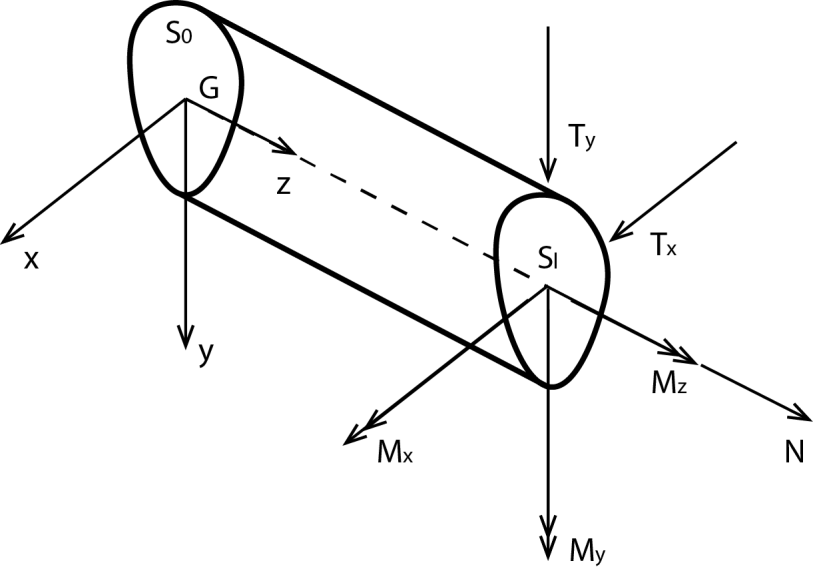
\includegraphics[width=0.7\linewidth]{fig/screenshot002}
		\caption{La successione di ruote ivi rappresentata è in ordine di complessità sia di analisi che di cinematismo.}
		\label{fig:screenshot002}
	\end{figure}
	
\newpage
	
	\begin{figure}[H]
		\centering
		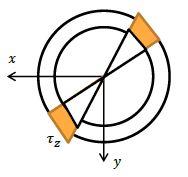
\includegraphics[width=0.8\linewidth]{fig/screenshot001}
		\label{fig:screenshot001}
	\end{figure}
	
	Si possono distinguere gli \textbf{ingranaggi cilindrici} in base sia alla posizione della dentatura sulla corona, che alla forma della dentatura, infatti possono essere
	\begin{itemize}
		\item A dentatura esterna
		
		La velocità di rotazione della ruota e del pignone sono opposte, una gira in senso orario mentre l'altra in senso antiorario.
		\begin{itemize}
			\item Dentatura dritta
			
			Lo sviluppo del profilo del dente è un estrusione nella direzione assiale di rotazione.
			
			\item Dentatura elicoidale 
			
			Lo sviluppo del profilo del dente avviene lungo un elicoide che si avvolge sul cilindro della primitiva.
			
			\item Dentatura bielicoidale
			
			È una ripetizione a specchio della seconda tipologia, per metà dello sviluppo assiale lo sviluppo del dente segue un'elicoide in una direzione, per l'altra metà segue un'elicoide in un'altra direzione.
		\end{itemize}
		\item A dentatura interna
		
		Le velocità di rotazione sono dello stesso verso.
	\end{itemize}

	Nel caso di treni di ingranaggi cilindrici, se gli assi di rotazione sono fissi, si osserverà una semplice successione di ingranaggi cilindrici in cui almeno un asse è in moto relativo rispetto agli altri, se invece TUTTI gli assi sono mobili quindi si avrà di fronte un ingranaggio di tipo \textbf{epicicloidale}.
	
	In un ingranaggio epicicloidale è composto da una ruota centrale, una corona esterna con dentatura interna e un portatreno che alloggia un certo numero di satelliti o ruote planetarie; a seconda che si vada a bloccare uno dei tre elementi costituivi, si ottiene in output un diverso rapporto di trasmissione. Il più classico dei cambi automatici a convertitore di coppia funziona attraverso ingranaggi epicicloidali. Anche la trasmissione delle vetture ibride Toyota si basa su ingranaggi di questo tipo: a seconda di cosa viene frenato tra portatreno, anello o ruota interna, si ottiene un flusso di energia dal motore a combustione interna verso le ruote, oppure dal MCI verso le batterie, oppure dalle batterie alle ruote. 
	
	I normali cambi di velocità manuali lavorano invece attraverso treni di ingranaggi cilindrici: quando si va ad innestare una marcia si innesta una determinata coppia di ingranaggi che vengono ad uno ad uno attivati, Il resto degli ingranaggi presenti sugli alberi sono invece resi folli, per cui quando si va ad innestare una marcia si va a disattivare (rendere folle) un ingranaggio, e ad attivarne un altro per renderlo solidale con l'albero in uscita. \newline
	
	Gli \textbf{ingranaggi conici} sono a loro volta classificati in funzione della posizione degli assi e della denatura
	\begin{itemize}
		\item Assi incidenti
		\begin{itemize}
			\item Dentatura dritta
			\item Dentatura obliqua (Gleason, Zerol)
		\end{itemize}
		\item Assi sghembi
		\begin{itemize}
			\item Dentatura ipoide
		\end{itemize}
	\end{itemize}
	Si possono trovare anche \textbf{ruote cilindriche ad assi sghembi}, dove il moto avviene tramite lo scambio di forze tra i profili dei denti, oppure si può individuare un accoppiamento \textbf{ruota-vite senza fine}: questo è l'elemento più complesso nella trattazione degli ingranaggi, il problema di questo tipo di accoppiamenti risiede nell'individuazione della superficie di contatto perché si tratta di superfici a doppia curvatura estremamente complesse, tuttavia questa soluzione è di estremo interesse ingegneristico perché permette la trasmissione del moto esattamente a 90\degree gradi occupando pochissimo spazio, è una soluzione usualmente utilizzata per movimentare i flap sull'ala di un aereo. 
\end{adjustwidth}

\subsection{Scelta}
\begin{adjustwidth}{2in}{}
	Come si sceglie tra una tipologia e l'altra? 
	
	Sicuramente entrano nei criteri di scelta lo spazio a disposizione, il livello tecnologico e quindi le efficienze ed il rapporto di trasmissione tipico.
	\begin{figure}[H]
		\centering
		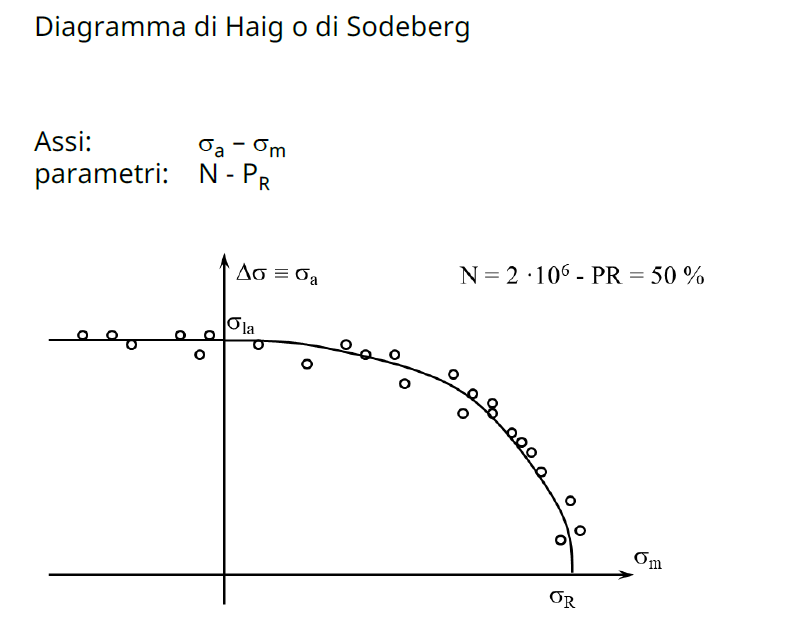
\includegraphics[width=0.7\linewidth]{fig/screenshot003}
		\label{fig:screenshot003}
	\end{figure}
	Come si vede dalla tabella le prime soluzioni hanno efficienze altissime, e sono ruote dentate cilindriche ad assi paralleli e ruote dentate coniche.
	
	Per le \textbf{ruote cilindriche} (argomento del corso), come ricade la scelta tra una dentatura dritta ed una elicoidale? 
	
	L'efficienza è riportata tra il 98\% e il 99\% per entrambi i casi.
	
	In realtà l'efficienza dipende dalla potenza in gioco e quindi dal momento torcente da trasmettere e quindi dalla velocità di rotazione e di conseguenza dal rapporto di trasmissione, tuttavia si può generalmente dire che di fronte ad una ruota dentata cilindrica a denti dritti l'efficienza è molto vicina al 99\% mentre per quelle a denti elicoidali si attesta intorno al 98\%.
	
	Tuttavia si possono ottenere rapporti di trasmissione decisamente più elevati con le ruote a denti elicoidali (10:1), rispetto a quelle a denti dritti (6:1), sempre facendo attenzione che quello in tabella è il rapporto di trasmissione ottenibile dalla singola coppia di ruote, se si utilizza un treno di ingranaggi il rapporto di trasmissione finale sarà sempre il prodotto del rapporto dei singoli ingranaggi. 
\newpage	
	Le \textbf{ruote coniche} hanno il grande vantaggio di trasferire il moto a 90\degree su assi incidenti, e al tempo stesso hanno un ottimo rendimento, di contro il rapporto di trasmissione trasmissibile è molto più basso.
	
	Se si deve garantire un rapporto di trasmissione elevato e si ha l'esigenza di trasferire il moto a 90\degree, si accoppierà nel riduttore un ingranaggio conico con uno cilindrico a cascata, uno dopo l'altro. \newline 
	
	In tabella sono presenti tutte le altre soluzioni caratterizzate da una grande variabilità di efficienza a seconda della disposizione degli assi, si può addirittura avere un'efficienza del 20\% in una coppia ruota vite senza fine con un rapporto di trasmissione fino a 75:1. 
	
	Si osserva così un trend che accoppia ad efficienze basse alti rapporti di trasmissione, come nelle ruote ipoidi e cicloidi. \newline 
		
	La scelta del tipo di ingranaggio deve essere ponderata anche sui costi: similmente ai cuscinetti, anche per le ruote dentate si ricorre a produzioni in serie da parte di aziende specializzate che possiedano le giunte tecnologie atte a mantenere determinati standard normati, per cui la scelta delle ruote dentate avviene sempre attraverso dei parametri normati come può essere quello del "\textit{proporzionamento modulare}".\newline 
	
	La scelta invece tra denti dritti e denti elicoidali prende in considerazione l'efficienza, i costi di realizzazione e la rumorosità, che fin'ora non era mai stata trattata. 
	
	Quell'1\% di efficienza in più delle ruote dentate a denti dritti è a fronte di un'elevata rumorosità dell'ingranaggio. 
	
	Le ruote dentate a denti elicoidali hanno di contro un punto percentuale di efficienza in meno, ma permettono un ingranamento  più silenzioso. 
\end{adjustwidth}

\section{Nomenclatura}
\begin{adjustwidth}{2in}{}
	In generale, il problema del progetto di una coppia di ingranaggi è legato da un lato all’aspetto geometrico-cinematico, dall’altro alla resistenza meccanica ed alla durata.

Si scinderanno i due concetti e si affronteranno separatamente, prima si studieranno gli aspetti geometrico-cinematici da dover rispettare per un corretto funzionamento dell'ingranaggio e poi a valle si faranno le corrette valutazioni di resistenza della dentatura.

Le verifiche da effettuare saranno in cascata: prima si verificheranno gli aspetti funzionali dimensionando effettivamente la ruota dentata e poi si effettueranno delle valutazioni di tipo resistenziale, in queste fase si eseguirà un procedimento di calcolo iterativo, per cui partendo da una considerazione di resistenza approssimata di primo tentativo, si effettueranno le verifiche geometrico-funzionali ed infine una verifica di dettaglio a resistenza della denatura attraverso modelli predefiniti. 
\end{adjustwidth}
\subsection{Nomenclatura generale}
\begin{adjustwidth}{2in}{}
	\begin{itemize}
		\item \textbf{Ingranaggio}: coppia di ruote dentate che in ingranano tra loro mediate il contatto tra i denti che vengono realizzati su di esse
		\begin{itemize}
			\item \textbf{Pignone}: della coppia, ruota di minor dimensione e con minor numero di denti.
			\item \textbf{Ruota}: della coppia, ruota di maggior dimensione e con maggior numero di denti.
		\end{itemize}
		\item \textbf{Riduttore}: La velocità della ruota condotto è minore di quella motrice (velocità in uscita minore di quella in entrata).
		\item \textbf{Moltiplicatore}: la velocità della ruota condotta è maggiore di quella motrice (velocità in uscita maggiore della velocità in entrata).
\newpage
		\item \textbf{Rotismo}, \textbf{Treno di ingranaggi}: serie di ingranaggi in successione per funzione di trasmissione del moto.
		\begin{itemize}
			\item \textbf{Ordinario} se ad assi fissi
			\item \textbf{Epicicloidale} se almeno un asse è mobile
		\end{itemize}
	\end{itemize}
\end{adjustwidth}



\subsection{Nomenclatura geometrica} 
\begin{adjustwidth}{2in}{}
	\begin{itemize}
		\item \textbf{Superfici primitive}
		
		\begin{deff} (Superfici primitive)
			
			Superfici descritte dall’asse di istantanea rotazione del movimento relativo della ruota coniugata rispetto alla ruota considerata.
		\end{deff} 
		Il moto tra le ruote dentate è descritto dalle superfici primitive. 
		
		\begin{deff} (Polare fissa \& Polare mobile)
			
			In un cinematismo si dice \textbf{polare fissa} l'insieme delle posizioni nel piano dei centri di spostamento e nello spazio degli assi di rotazione - entrambi istantanei - che questo asse assume nel sistema di riferimento fisso globale.
			
			La \textbf{polare mobile} è invece la curva nel piano, o superficie nello spazio, che descrive le posizioni nel sistema di riferimento mobile degli assi di istantanea rotazione.
		\end{deff}
		Polare fissa e polare mobile rappresentano le posizioni nel tempo che assume l'asse di istantanea rotazione. \newline
		
		Ciascuna primitiva nel moto relativo di una rispetto all'altra assume il ruolo di polare fissa e di polare mobile. \newline
		
		Le polari - o superfici primitive - fanno parte dell'accoppiamento cinematico, ovvero ne descrivono il cinematismo, ma sono entità cinematiche non misurabili fisicamente sull'ingranaggio.
		\begin{figure}[H]
			\centering
			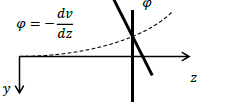
\includegraphics[width=0.3\linewidth]{fig/screenshot004}
			\label{fig:screenshot004}
		\end{figure}
		Al contrario, i denti sono elementi fisici misurabili che in parte sporgono e in parte rientrano dalla primitiva, questo perché il moto di perfetto rotolamento senza strisciamento avviene soltanto sulla polare, perciò quando avviene il contatto in punti che non fanno parte della polare non si verifica più il puro rotolamento bensì un rotolamento con strisciamento, di conseguenza sarà necessario distribuire spazialmente il dente a cavallo della primitiva cosi da limitare lo strisciamento fra denti mutuamente ingranati.
		
		\item \textbf{Superficie di testa}
		\begin{figure}[H]
			\centering
			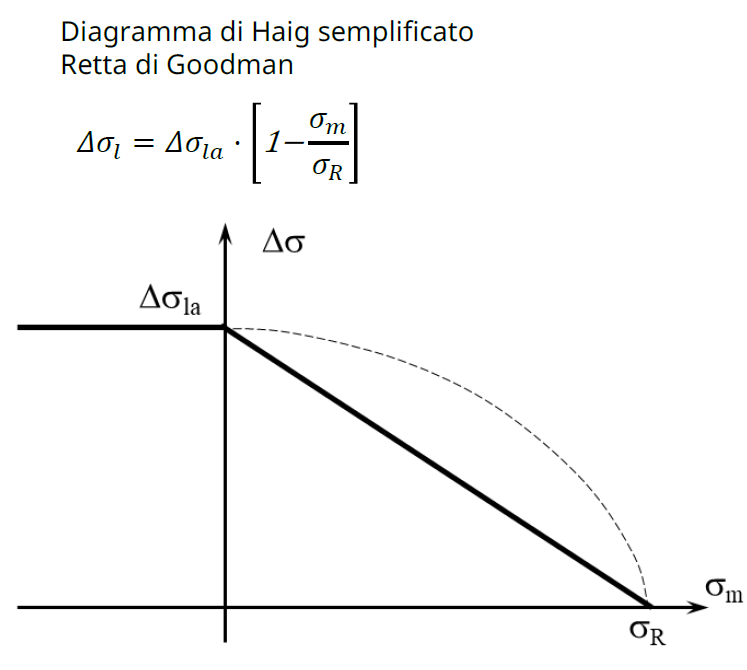
\includegraphics[width=0.3\linewidth]{fig/screenshot005}
			\label{fig:screenshot005}
		\end{figure}		
		Superficie coassiale alla ruota, che contiene la sommità dei denti, la loro parte più sporgente.
\newpage		
		\item \textbf{Superficie di piede}
		\begin{figure}[H]
			\centering
			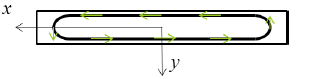
\includegraphics[width=0.3\linewidth]{fig/screenshot006}
			\label{fig:screenshot006}
		\end{figure}
		Superficie coassiale alla ruota che contiene il fondo dei denti. \newline
		
		\textbf{La superficie di piede non deve mai esser confusa con la superficie di base che si vedrà vere un significato diverso.}
		
		\item \textbf{Fianco}
		\begin{figure}[H]
			\centering
			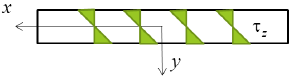
\includegraphics[width=0.3\linewidth]{fig/screenshot007}
			\label{fig:screenshot007}
		\end{figure}
		Porzione di dente compresa tra la superficie di testa e la superficie di piede.
		
		\item \textbf{Linea di fianco}
		\begin{figure}[H]
			\centering
			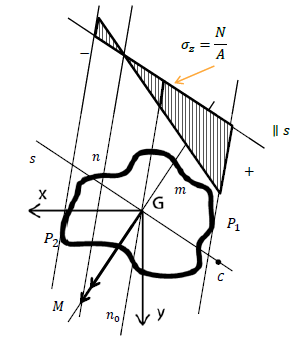
\includegraphics[width=0.3\linewidth]{fig/screenshot008}
			\label{fig:screenshot008}
		\end{figure}
		Segmento - individuabile sul fianco - intersezione tra il fianco del dente e la superficie primitiva.
		
		\item \textbf{Profilo}
		\begin{figure}[H]
			\centering
			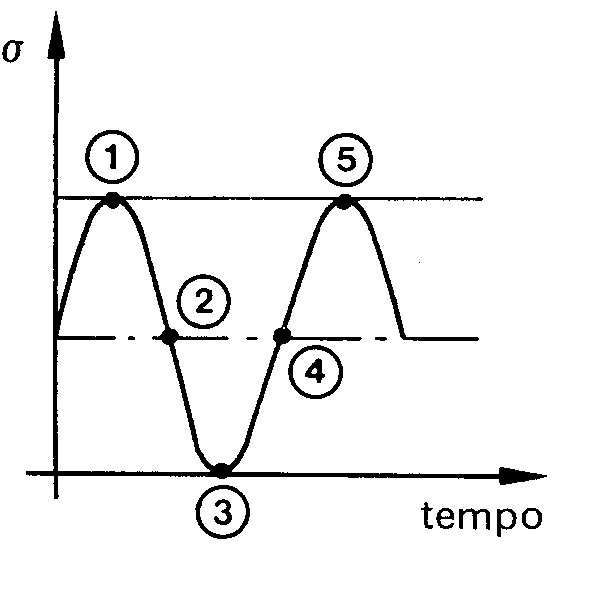
\includegraphics[width=0.3\linewidth]{fig/screenshot009}
			\label{fig:screenshot009}
		\end{figure}
		Intersezione del fianco del dente con un piano ortogonale all'asse di rotazione.
		
\newpage

		\item \textbf{Dente dritto VS Dente elicoidale}
		\begin{figure}[H]
			\centering
			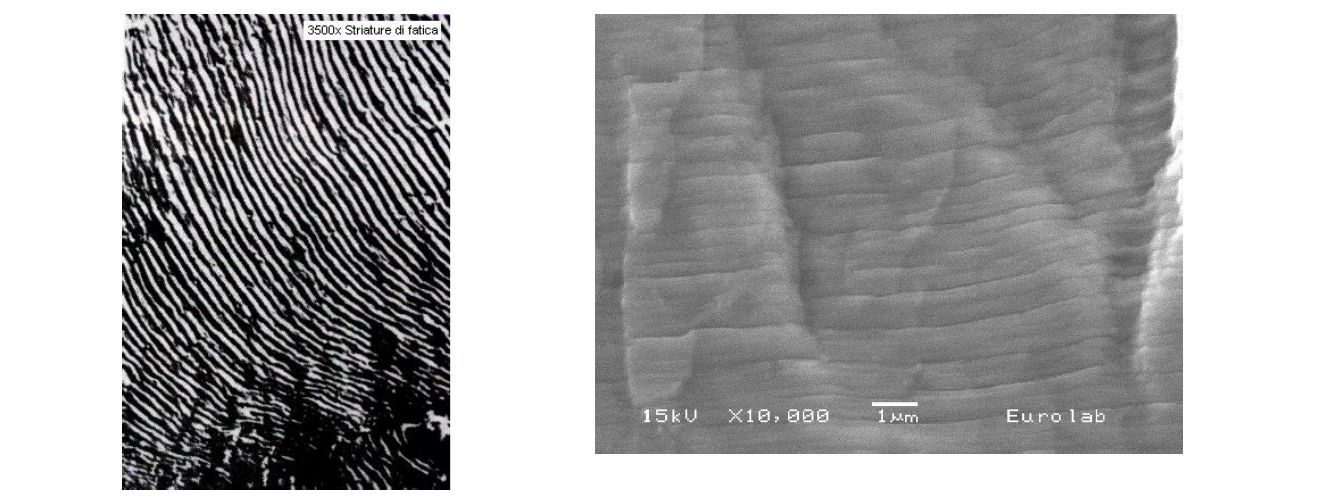
\includegraphics[width=0.5\linewidth]{fig/screenshot010}
			\label{fig:screenshot010}
		\end{figure}
		Sempre nel caso di superficie primitiva cilindrica si parla di
		\begin{itemize}
			\item \textbf{Dente dritto} se la superficie di fianco del è ottenuta per estrusione del profilo del dente nella direzione dell'asse di rotazione (che combacia con la direzione assiale per ruote cilindriche).
			\item \textbf{Dente elicoidale} se il fianco del dente è ottenuto mediante un estrusione del profilo del dente lungo un elica che si avvolge sulla circonferenza, sul cilindro primitivo.			
		\end{itemize}
		In sostanza, il primo è un estrusione del profilo lungo l'asse della ruota mentre l'altro è un estrusione che avviene lungo un elica disegnata su una superficie cilindrica.		
	\end{itemize}
\end{adjustwidth}	
	
\subsection{Nomenclatura cinematica}
\begin{adjustwidth}{2in}{}
	\begin{itemize}
		\item \textbf{Profilo attivo}: fianco del dente effettivamente in contatto con la ruota coniugata.
		\begin{figure}[H]
			\centering
			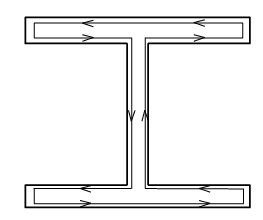
\includegraphics[width=0.15\linewidth]{fig/screenshot011}
			\label{fig:screenshot011}
		\end{figure}
		\item \textbf{Profilo ozioso}: fianco del dente che NON entra a contatto con la ruota coniugata		
		\end{itemize}
		Questa distinzione si fonda sul fatto che ad un ingranaggio si può imporre un moto di rotazione invertito, allo stesso tempo però il cinematismo di trasferimento di potenza si avrà solo e soltanto in un verso, quindi mentre sussiste un certo regime di rotazione, ci sarà sempre un fianco in contatto con il dente coniugato ed un fianco totalmente inutilizzato. \newline 
		
		La geometria del dente deve naturalmente rispondere ad esigenze tecnologiche di realizzazione e di resistenza, si individuano teste e radici che spaziano successivi profili oziosi e attivi.	
		\begin{itemize}
			\item \textbf{Radice}: parte inferiore del dente che non fa parte del profilo.
			\begin{figure}[H]
				\centering
				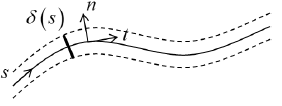
\includegraphics[width=0.15\linewidth]{fig/screenshot012}
				\label{fig:screenshot012}
			\end{figure}
			Per la radice del dente passa la circonferenza di piede.
\newpage
			\item \textbf{Testa}: parte superiore del dente che non fa parte del profilo.
			\begin{figure}[H]
				\centering
				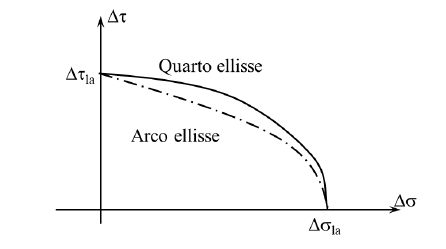
\includegraphics[width=0.15\linewidth]{fig/screenshot013}
				\label{fig:screenshot013}
			\end{figure}			
			Per la testa del dente passa la circonferenza di testa.
			
			\item \textbf{Raccordi di piede \& di testa}
			\begin{figure}[H]
				\centering
				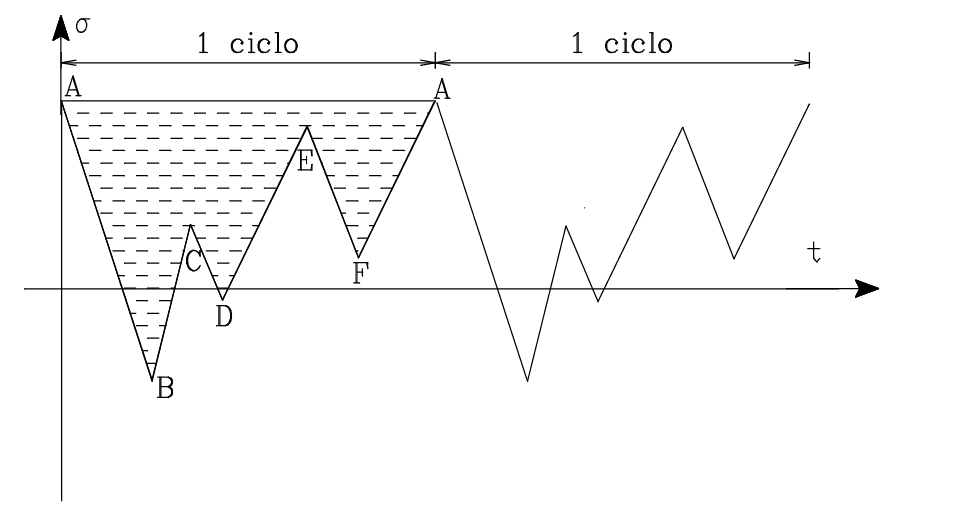
\includegraphics[width=0.15\linewidth]{fig/screenshot014}
				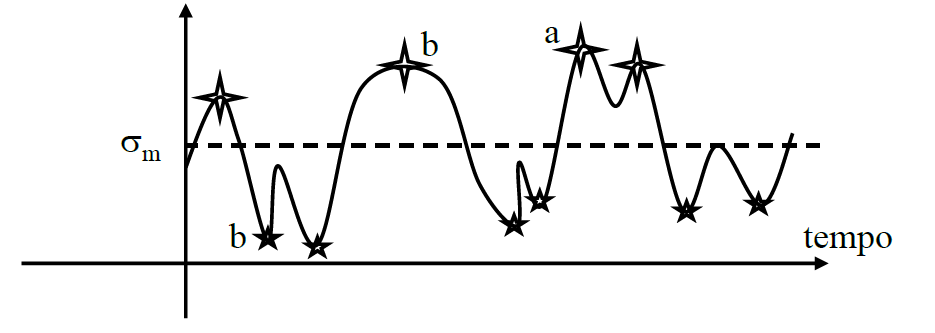
\includegraphics[width=0.15\linewidth]{fig/screenshot015}
				\label{fig:screenshot014}
			\end{figure}			
			Per evitare l'effetto delle concentrazioni di tensione ci sono sempre sempre un raccordo di piede ed un raccordo di testa, anche se quest'ultimo non è obbligatorio.			
		\end{itemize}
		
	\begin{deff}(Profili coniugati)
		
		Due profili si dicono coniugati se la normale comune nel punto
		di contatto passa per il centro di istantanea rotazione, che, in
		questo caso, è il punto di tangenza tra le due primitive. \newline 
		
		I profili si dicono coniugati se instante per instante durante il funzionamento, la normale comune ai due profili, passa per l'asse di istantanea rotazione. \newline
	\end{deff}
	
	Allora per funzionare e avere moto continuo ruota e pignone dovranno avere due profili attivi di tipo coniugato.
	
	Due sono le indicazioni
	\begin{enumerate}
		\item \textbf{Le normali devono essere comuni}
		
		Ciò è di vitale importanza perché significa dire che i profili devono essere delle curve tangenti nel punto di contatto, se così non fosse l'ingranamento avverrebbe in maniera non corretta, magari con strisciamenti.
		
		\item \textbf{La normale passa per l'asse di istantanea rotazione}
		
		Se così non fosse i profili non sarebbero più coniugati.		
	\end{enumerate}
\newpage

	\begin{figure}[H]
		\centering
		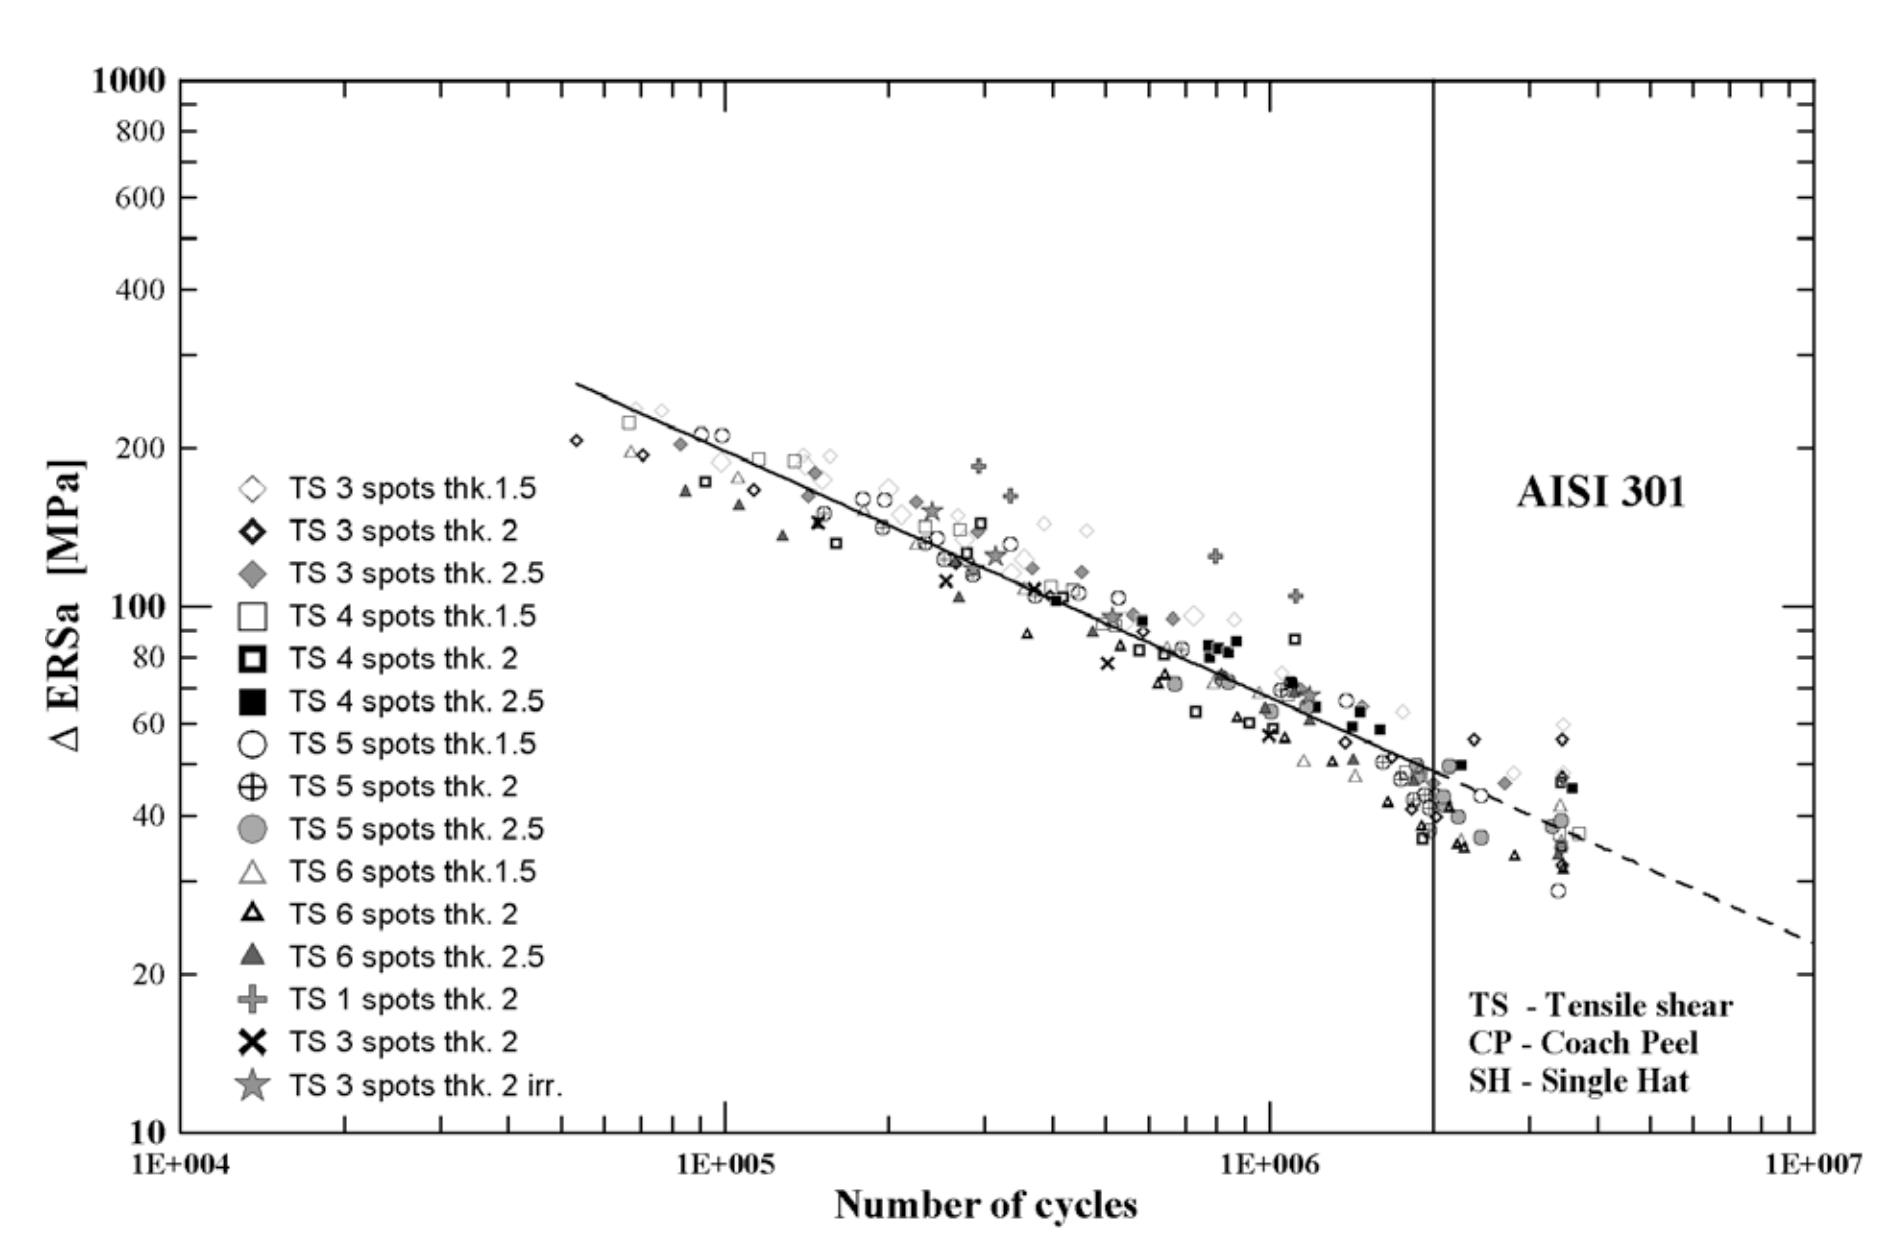
\includegraphics[width=0.7\linewidth]{fig/screenshot016}
		\label{fig:screenshot016}
	\end{figure}
	\begin{itemize}
		\item \textbf{Spessore}: distanza misurata sulla superficie della circonferenza primitiva tra due profili attivo ed ozioso appartenenti allo stesso dente.
		
		Misurato come arco di circonferenza primitiva.
		
		\item \textbf{Vano}: misura dello spazio tra il profilo ozioso ed il profilo attivo del dente successivo.
		
		Misurato come arco di circonferenza primitiva.
		
		\item \textbf{Passo}:distanza, sempre misurata come arco di circonferenza primitiva, tra due profili attivi successivi appartenenti a due denti successivi.
		
		Il passo sarà dato dalla somma dello spessore del dente e del vano della ruota.
		
		\item \textbf{Altezza}: distanza radiale tra la testa e la radice del dente, distanza radiale tra la superficie di testa e la superficie di piede.
		
		\item \textbf{Addendum \& Dedendum}
		
		L'altezza del dente è distribuita intorno alla superficie primitiva, a cavallo di essa, il dente quindi sporgerà rispetto alla circonferenza primitiva di un \underline{addendum} mentre rientrerà rispetto alla circonferenza primitiva di un \underline{dedendum}.
		
		La somma di addendum e dedendum dà l'altezza totale del dente.		
	\end{itemize}
\end{adjustwidth}
	\begin{figure}[H]
		\centering
		\includegraphics[width=0.7\linewidth]{fig/156}
		\caption{}
		\label{fig:156}
	\end{figure}
	
\newpage
\section{Moto relativo}
\begin{adjustwidth}{2in}{}
	Due ruote dentate hanno un moto relativo descrivibile come il rotolamento senza strisciamento di una superficie primitiva sull'altra.
	
	Nel caso delle ruote più semplici, quelle cilindriche, si avranno due cilindri che rotolano senza strisciare l'uno sull'altro, se nel punto di tangenza - o linea di tangenza - si fa passare un piano tangente alle due superfici, si potrà immaginare il moto come se questo fosse generato dall'azione di tirare il piano tangente individuato.
	\begin{figure}[H]
		\centering
		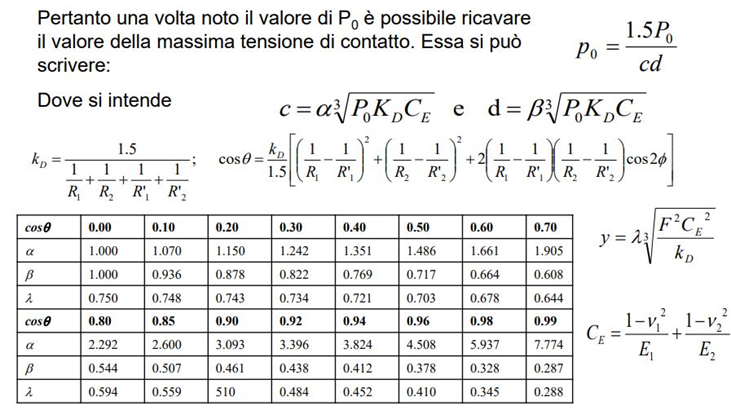
\includegraphics[width=0.5\linewidth]{fig/screenshot017}
		\label{fig:screenshot017}
	\end{figure}
	Tirando il piano in una direzione si verifica un moto di rotazione dei due cilindri primitivi che rotolano senza strisciare l'uno sull'altro.\newline
	
	\begin{en}
		Le velocità di rotazione $\omega_1$ e $\omega_2$ sono sia di verso che di valore opposto.
	\end{en}
	\begin{proof}
		Un punto sul cilindro 1 che appartiene al punto $C$ ovvero alla traccia dell'asse di istantanea rotazione in un piano ortogonale agli assi sarà dotato di velocità $v_t = \omega_1r_1$, allo stesso modo il punto della ruota 2 che in quell'istante di tempo si trova anch'esso in $C$, è è caratterizzato dalla stessa velocità periferica $v_t = \omega_2r_2$, infatti poiché il moto è di rotolamento senza strisciamento vuol dire che nel punto $C$ la velocità istantanea relativa è nulla, e quindi le velocità istantanee assolute dovranno essere giocoforza identiche, per cui
		\[v_t = \omega_1r_1 = \omega_2r_2\] 
		E quindi
		\[ \dfrac{\omega_1}{\omega_2} = \dfrac{r_2}{r_1}\]
		In un ingranaggio il rapporto tra le velocità di rotazione è inversamente proporzionale al rapporto fra i raggi, il che vuol dire che per avere una riduzione del 50\% della velocità in uscita si deve necessariamente avere una ruota grande il doppio: se l'obiettivo è una velocità in uscita la meta di quella in ingresso, si dovrà avere una ruota condotta il doppio di quella motrice.
	\end{proof}
\end{adjustwidth}
\newpage
\subsection{Trasmissione del moto}
\begin{adjustwidth}{2in}{}	 
	Il requisito fondamentale che la geometria del profilo del
	dente dell'ingranaggio deve soddisfare è la garanzia di un
	rapporto di trasmissione esattamente costante.\newline 
	
	Questo requisito è soddisfatto dalla condizione di coniugio del dente ovvero i profili delle ruote dentate devono essere coniugati.	
	\begin{figure}[H]
		\centering
		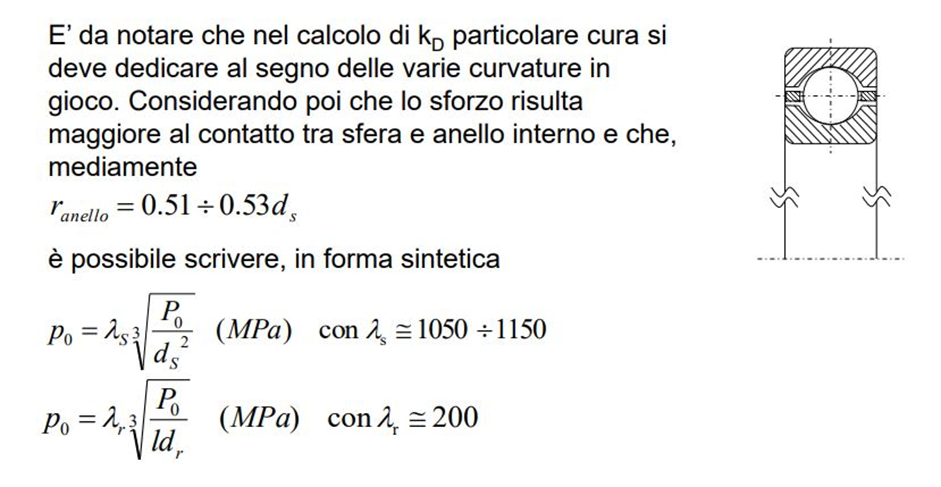
\includegraphics[width=0.45\linewidth]{fig/screenshot018}
		\label{fig:screenshot018}
	\end{figure}	
	Due denti in reciproco contatto possono essere visti come due semplici leve. 
	
	Si può da subito individuare un punto di contatto $P$. 
	
	Naturalmente i profili di queste due leve sono coniugati perché la loro normale nel punto di contatto è comune ai due, ciò vuol dire che nel punto di contatto le superfici sono tangenti e questa normale punta esattamente nel centro di istantanea rotazione, che nel caso di una ruota cilindrica si trova esattamente sull'interasse tra le due ruote e rimane fermo nel tempo.
	
	D'ora in avanti per le ruote dentate cilindriche si può lavorare su un piano trasversale agli assi, e quindi riportare il cinematismo ad un problema bidimensionale senza dover ogni volta rappresentare tridimensionalmente l'ingranaggio.\newline
	
	La normale comune è detta \textbf{linea d'azione} e da $P$ passa per $C$, lungo questa retta avviene l'applicazione delle forze scambiate.
	
	Questo perché le forze vengono trasmesse mediante semplice contatto e ciò è sempre espresso - ad eccezione degli aspetti d'attrito - nella direzione ortogonale ai profili, per questo la componente di forza scambiata è nella direzione della linea d'azione.
\end{adjustwidth}
\newpage
\section{Profilo ad evolvente}
\begin{adjustwidth}{2in}{}	
	Tra i possibili profili coniugati il più utilizzato è quello ad evolvente di circonferenza.
	
	Questo particolare profilo coniugato possiede una serie di proprietà estremamente importanti, prima fra tutte, l'inclinazione della linea d'azione rimane costante durante tutto l'ingranamento, durante tutto l'arco di rotazione durante il quale i denti sono in presa: la linea d'azione rimane inclinata di un certo \textbf{angolo di pressione} $\theta$ sempre costante. \newline
	
	Tuttavia si nota dai disegni che il punto $P$ di contatto tra i profili non è appartenente alle circonferenze primitive e quindi sarà un punto di contatto strisciante. 
	
	Ciò si può vedere chiaramente dalla distribuzione dei vettori velocità in quel punto.
	\begin{figure}[H]
		\centering
		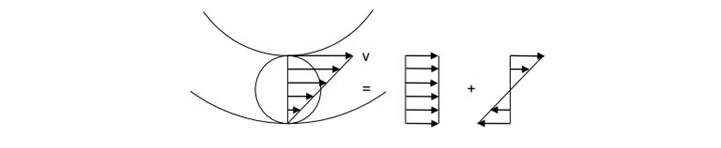
\includegraphics[width=0.65\linewidth]{fig/screenshot019}
		\label{fig:screenshot019}
	\end{figure}
	In P la velocità del punto del profilo in contatto appartenente col dente della ruota 1 $v_{P1}$, è una velocità periferica dettata dal moto di rotazione della ruota, in assenza di compenetrazioni o deformazioni eccessive, questa è sempre esprimibile come $v_{P1} = \omega_1r_1$ ed è orientata (essendo un modo di rotazione) ortogonalmente al vettore posizione radiale $r_{P1}$; al tempo stesso però il punto in contatto è comune alle due ruote, e quindi per la seconda ruota varrà giocoforza $v_{P2} = \omega_2r_2$ con direzione ortogonale al vettore posizione radiale $r_{P2}$. \newline
	
	Tuttavia questi vettori hanno - per intrinseca caratteristica dell'evolvente e per il fatto di essere coniugati - la stessa componente di velocità nella direzione ortogonale al profilo: $v_{n1} = v_{n2}$.
	
	Infatti per garantire continuità del moto i due profili, da quando inizia a quando finisce il contatto, rimangono sempre tra loro uniti in un punto, ciò vuol dire che nell'avanzamento dei due profili non c'è mai nè separazione nè compenetrazione degli stessi, e quindi nella direzione ortogonale al profilo la velocità si mantiene per forza costante, analogamente ciò è intuibile dal fatto che la ruota motrice si porta sempre dietro la condotta alla stessa distanza nella direzione ortogonale al profilo, ciò vuol poter dire solo che che la componente $v_n$ è la medesima.\newline
	
	Dato che i denti hanno velocità differenti l'ingranaggio è sempre portato a strisciamenti, poiché si è appena visto che la componente di velocità normale al dente è costante, gli strisciamenti saranno allora per forza dovuti alla componente della velocità tangenziale al profilo del dente $v_t$ e ciò porta inevitabilmente a fenomeni di usura e pitting.
\end{adjustwidth}
\newpage
\subsection{Dentatura ad evolvente}
\begin{adjustwidth}{2in}{}
	 Il contatto tra i profili del dente in una dentatura ad evolvente avviene lungo una retta che ricalca esattamente la linea d'azione: i punti di contatto sul profilo del dente si muovono in un piano ortogonale all'asse lungo la linea d'azione, che ora prende il nome di \textbf{linea dei contatti}.
	 \begin{figure}[H]
	 	\centering
	 	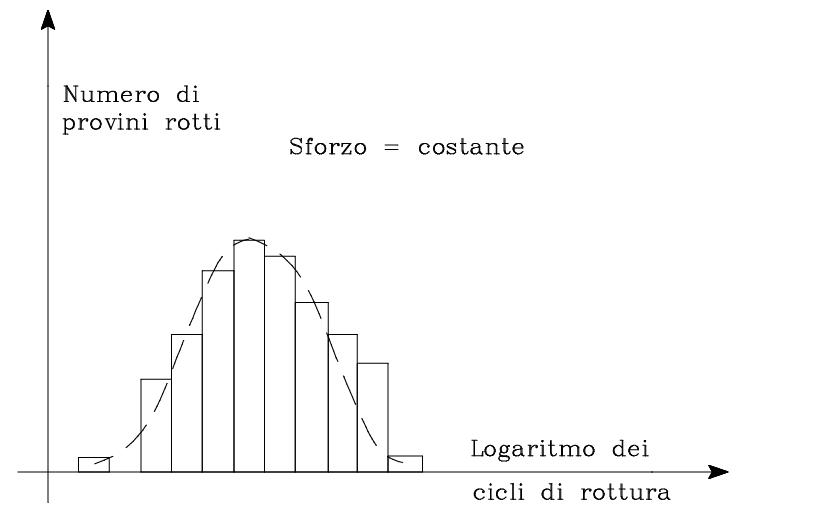
\includegraphics[width=0.65\linewidth]{fig/screenshot020}
	 	\label{fig:screenshot020}
	 \end{figure}	 
	 Quando il pignone ruota di velocità $\omega_1$ costringendo la ruota a ruotare di velocità $\omega_2$, il dente del pignone tocca il dente della ruota in un primo punto $P_1$: la parte bassa del dente 1 tocca la testa del dente 2, questo punto giace proprio sulla linea d'azione (dei contatti) che rimane inclinata sempre dell'angolo di pressione $\theta$.
	 
	 Negli istanti successivi al primo contatto, durante la rotazione, l'ingranamento avverrà in punti successivi, tra questi ci sarà il punto $C$ di istantanea rotazione. 
	 
	 A questo punto l'ingranamento continua fino al punto $P_2$, ultimo punto utile di contatto: finisce il profilo del pignone. \newline 
	 
	 La retta dei contatti risulta così rispettivamente tangente ad una circonferenza per la ruota e ad un'altra per il pignone, queste due circonferenze $c_b$, il cui raggio viene spesso indicato con la lettera $\rho$, sono dette \textbf{circonferenze base} o \textbf{circonferenze fondamentali dell'evolvente} e sono grandezze caratteristiche della dentatura della ruota e del pignone.
	 
	 I punti di tangenza delle circonferenze fondamentali con la retta d'azione, $T_1$ e $T_2$ rappresentano gli ultimi punti possibili di contatto tra ruota e pignone.\newline
	 
	 Poiché il profilo ad evolvente si sviluppa a partire dalla circonferenza fondamentale, ovvero non può esistere profilo ad evolvente al di sotto della circonferenza fondamentale, la forma ad evolvente parte dalla circonferenza fondamentale e si sviluppa radialmente verso la circonferenza di testa, ciò vuol dire che il primo punto utile per l'ingranamento, ovvero il primo punto utile per avere profili coniugati è proprio $T_1$, ed il segmento $T_1T_2$ - ovvero l'estensione dei potenziali punti di contatto dal primo punto utile sul pignone all'ultimo punto utile sulla ruota - viene chiamato \textbf{segmento massimo}  o \textbf{teorico dei contatti}. \newline
	 
	 Nella realtà il \textbf{segmento effettivo dei contatti} è molto più piccolo ed è individuato da $P_1P_2$ e sarà dettato dalle circonferenze di troncatura esterna di ruota e pignone.
\newpage	 
	 Le \textbf{circonferenze di troncatura} esterna e interna si differenziano dalle circonferenze di testa e di piede perché queste ultime vengono ricavate al netto dei raccordi di testa e di piede del dente; vuol dire che nel profilo, data una circonferenza di testa dove si avrà un angolo di spoglia e quindi un raggio di raccordo, la circonferenza di troncatura esterna sarà più bassa della circonferenza di testa e terrà conto del raggio di raccordo (che non prende parte ai contatti), simile per la troncatura interna, più alta della troncatura di base e terrà conto del raccordo di base che non prenderà parte ai contatti (nella figura (\ref{fig:156}) è chiamata "circonferenza del gioco"). 
	 
	 Si definisce in questo modo l'entità del profilo utile al contatto cioè quella parte di profilo che effettivamente è a forma di evolvente. \newline	 	 
	 
	 \begin{deff}(Arco d'azione)
	 	
	 	Arco, misurato sulla primitiva, durante il quale rimangono in contatto due
	 profili coniugati. \newline
	 \end{deff}
	 
	 Quando il contatto inizia in $P_1$ il profilo del dente del pignone (ruota 1) interseca la superficie primitiva nel punto $A_1$, analogamente quando l'ingranamento volge al termine in $P_2$ il profilo del dente della ruota (ruota 2) interseca la circonferenza primitiva in $A_2$.
	 
	 La somma dell'arco $A_1C$ e dell'arco $CA_2$ rappresenta la lunghezza dell'arco d'azione.
	 
	 L'arco $A_1C$ è detto \textbf{arco di accesso}, l'arco $CA_2$ è detto \textbf{arco di recesso}. Per convenzione l'arco di accesso viene preso sul pignone, e quindi sulla ruota motrice nel caso di riduttore, mentre invece l'arco di recesso sulla ruota condotta, tuttavia per proprietà dell'evolvente e vista la mancanza di strisciamento nel cinematismo, si ottengono le stesse misure degli archi anche a ruote invertite. \newline
	 
	 L'arco di azione si può ottenere anche attraverso il segmento dei contatti.
	 
	 Per proprietà dei profili ad evolvente la linea dei contatti corrisponde alla linea d'azione ed è inclinata sempre dello stesso angolo di pressione $\theta$ per cui si può scrivere
	 \[A_1CA_2 = \dfrac{P_1P_2}{\cos\theta}\]
	 In questo modo la lunghezza dell'arco d'azione - che è difficile da ottenere in termini di misurazione di archi di circonferenza, si può ottenente per rapporto tra il segmento dei contatti - termine rettilineo - ed il coseno dell'angolo di pressione.
\end{adjustwidth}
\newpage
\subsection{Numero di denti}
	 \begin{figure}[H]
	 	\centering
	 	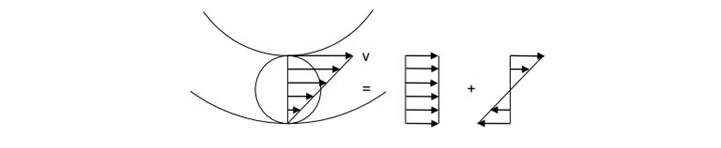
\includegraphics[width=0.65\linewidth]{fig/screenshot019}
	 	\label{fig:screenshot019_bis}
	 \end{figure} 
	 
\begin{adjustwidth}{2in}{}
	 È bene osservare che il generico punto di contatto $P$ si sposta sul segmento dei contatti con una velocità pari a quella periferica, calcolata sulle circonferenze fondamentali.\newline 
	 	 
	 Si è visto che per le proprietà degli evolventi il punto di contatto $P$ si muove sulla retta d'azione con una componente di velocità lungo la stessa (è la componente normale di qualche pagina fa) costante durante tutto l'ingranamento, questa velocità è pari alla velocità periferica nei punti $T_1$ e $T_2$, ovvero nei punti di tangenza della retta d'azione con la circonferenza fondamentale.
	 
	 Sapendo che 
	 \[\omega = \dfrac{v}{r} \] 
	 Allora in riferimento all'immagine tale rapporto dovrà rimanere costante sia che ci si trovi in $C$ o in $T_1$ o in $T_2$ o in $P_1$ o in $P_2$.
	 \[\begin{dcases}
	 	\omega_1 = \dfrac{v_{P1}}{r_{P1}} = \dfrac{v_1}{r_1} = \dfrac{v_{n1}}{r_{b1}} \\
	 	\omega_2 = \dfrac{v_{P2}}{r_{P2}} = \dfrac{v_2}{r_2} = \dfrac{v_{n2}}{r_{b2}}
	 \end{dcases}\]
	 Allora 
	 \[\begin{dcases}
	 	v_{n1} = v_1\dfrac{r_{b1}}{r_1} \\
	 	v_{n2} = v_2\dfrac{r_{b2}}{r_2}
	 \end{dcases}\]
	 La proporzione geometrica tra il raggio di primitiva $r$ e il raggio di base $r_b$ è dettata dal fatto che la retta dei contatti - di inclinazione $\theta$ - è ortogonale al raggio di base per costruzione, e allora l'angolo $\theta$ di inclinazione della retta d'azione è esattamente l'angolo che si interpone tra il raggio di primitiva e il raggio di base, e allora varrà 
	 \[\begin{dcases}
	 	v_{n1} = v_1\cos\theta\\
	 	v_{n2} = v_2\cos\theta
	 \end{dcases}\]
\newpage
	 Sostituendo e ricordando che per definizione di profilo coniugato tali velocità devono essere uguali nel punto di contatto per garantire continuità del moto si arriva a
	  \[\begin{dcases}
	 	v_1\cos\theta = v_1\dfrac{r_{b1}}{r_1} \\
	 	v_2\cos\theta = v_2\dfrac{r_{b2}}{r_2}
	 \end{dcases} \Rightarrow \cos\theta = \dfrac{r_{b1}}{r_1} = \dfrac{r_{b2}}{r_2} \]
	 Significa che il profilo coniugato garantisce un cinematismo dettato dalle sole primitive di rotolamento, il  rapporto che si instaura così tra le velocità $\omega_i$ si può riscrivere come 
	 \[\dfrac{\omega_1}{\omega_2} = \dfrac{v_1}{r_1}\dfrac{r_2}{v_2} = \dfrac{r_2}{r_1} = \dfrac{z_2}{z_1}\]
	 Dove si è introdotto il fatto che il numero di denti $z$ è proporzionale alle dimensioni della ruota, ciò alla sua circonferenza. \newline 
	 
	 La grandezza che tiene conto della proporzione tra la circonferenza e il numero di denti è il modulo trasversale $m$. 
\end{adjustwidth}

\subsection{Nomenclatura di riferimento}
\begin{adjustwidth}{2in}{}	 
	Le grandezze senza apice e con $pedice_1$ fanno riferimento alla ruota motrice, quelle con apice' e $pedice_2$ alla ruota condotta. 

		\begin{table}[H]
			\centering
		\begin{tabular}{|c|c|}
			\hline
			O \quad O'       & Centri geometrici delle ruote                                                                           \\ [0.85ex] \hline
			z \quad z'       & Numero di denti                                                                                         \\ [0.85ex] \hline
			R \quad R'       & Raggi primitivi                                                                                         \\ [0.85ex] \hline
			$\rho$ \quad $\rho$' & Raggi delle circonferenze di base della dentatura ad evolvente                                          \\ [0.85ex] \hline
			p                & \begin{tabular}[c]{@{}c@{}}Passo trasversale\\ $p = \dfrac{2\pi R}{z} = \dfrac{2\pi R'}{z'}$\end{tabular} \\ [0.85ex] \hline
			m                & \begin{tabular}[c]{@{}c@{}}Modulo trasversale\\ $m=\dfrac{2R}{z} = \dfrac{2R'}{z'}$\end{tabular}          \\ [0.85ex] \hline
							 & \begin{tabular}[c]{@{}c@{}}Notare come\\ $p = m\cdot\pi$\end{tabular} 										\\ [0.85ex] \hline
			a                & Addendum del dente                                                                                      \\ [0.85ex] \hline
			u                & Dedendum del dente                                                                                      \\ [0.85ex] \hline
			h                & Altezza del dente                                                                                      \\ [0.85ex] \hline
			$\Omega$ \quad $\Omega$'& Centri di curvatura dei profili nel punto di contatto \\ \hline
			$M\Omega$ \quad $M\Omega$' & Raggi di curvatura dei profili nel punto di contatto \\ \hline
			$\delta$ & \begin{tabular}[c]{@{}c@{}}Distanza del punto di contatto dal centro di istantanea rotazione $C$,\\ misurata sul segmento di contatto, varia nel tempo durante l'ingranamento.\end{tabular}  \\ \hline
			$\omega$ \quad $\omega$'& Velocità angolari delle ruote \\ \hline
			$\theta = \theta_0$ & Angolo di pressione \\ \hline
			s & Spessore del dente misurato sulla circonferenza primitiva \\ \hline
			e & Vano misurato sulla circonferenza primitiva \\ \hline
			$\varepsilon$ & \begin{tabular}[c]{@{}c@{}}Fattore di ricoprimento\\ $\varepsilon = \dfrac{\text{arco d'azione}}{p} = \dfrac{\text{segmento dei contatti}'}{p\cos\theta_0}$\end{tabular} 										\\ \hline 
		\end{tabular}
	\end{table}
\newpage

		È in particolare il fattore di ricoprimento a garantire continuità del moto, infatti lo si può vedere dall'immagine degli archi d'azione 
		\begin{figure}[H]
			\centering
			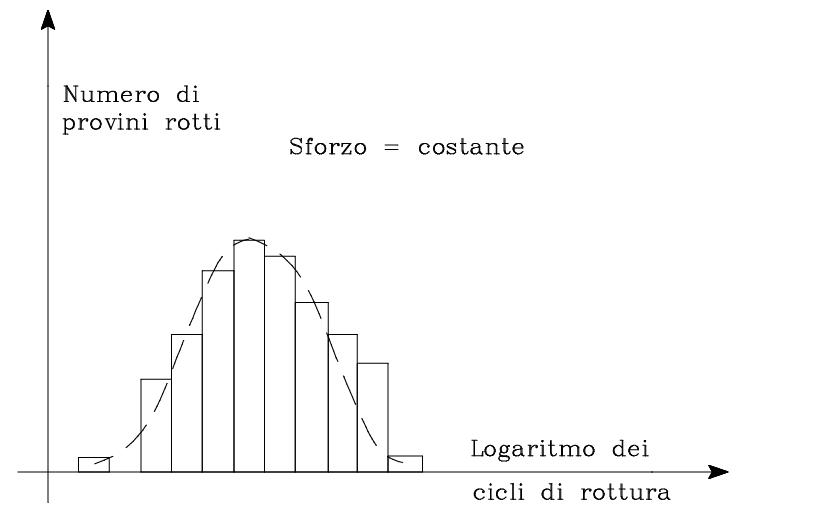
\includegraphics[width=0.5\linewidth]{fig/screenshot020}
			\label{fig:screenshot020_bis}
		\end{figure}		
		L'arco d'azione va da $A_1$ ad $A_2$, il passo è invece la distanza sulla circonferenza primitiva tra due profili attivi successivi, risulta quindi evidente come il passo debba essere lo stesso sia su ruota che su pignone, se infatti il passo fosse diverso si avrebbe un ingranamento non corretto. \newline
		
		Per verificare il corretto ingranamento si introduce così fattore di ricoprimento $\varepsilon$, questo è il rapporto tra arco d'azione e passo e dev'essere sempre maggiore all'unità: l'arco d'azione dev'essere sempre superiore al passo. 
		
		Se così non fosse e ad esempio il passo fosse più piccolo dell'arco, mentre la coppia di denti in presa sta finendo il suo ingranamento in $P_2$, avviene subito il contatto con un'altra coppia di denti (impuntamento); se invece il passo fosse maggiore dell'arco, significherebbe che in $P_2$, sempre alla fine dell'ingranamento, il successivo dente del pignone deve ancora arrivare e la ruota condotta rimane ferma ad aspettarlo, ciò significa avere un moto non continuo con urti. \newline
		
		Al fine di evitare questi effetti di impuntamento, urti e perdita di efficienza, il fattore di ricoprimento dev'essere almeno pari a 1.2$\div$1.4 a seconda della velocità di rotazione dell'ingranaggio. 
	\end{adjustwidth}
\newpage	
	\subsection{Profilo ad evolvente}
	\begin{adjustwidth}{2in}{}	
		Una curva ad evolvente di circonferenza è un profilo piano che viene descritto da un punto appartenente ad una retta che rotola senza strisciare su  una circonferenza fondamentale. 
		\begin{figure}[H]
			\centering
			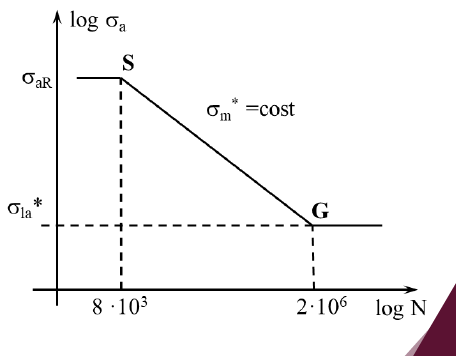
\includegraphics[width=0.3\linewidth]{fig/screenshot021}
			\label{fig:screenshot021}
		\end{figure}
		Al di sotto della circonferenza di base (o fondamentale) non esiste e non può esistere l'evolvente. 
		
		L'evolvente si traccia dalla circonferenza di base con una traiettoria iniziale che è perfettamente ortogonale alla circonferenza, per cui il primissimo tratto dell'evolvente è radiale, dopodiché come acquista distanza il profilo del dente diviene ad evolvente.
		\begin{figure}[H]
			\centering
			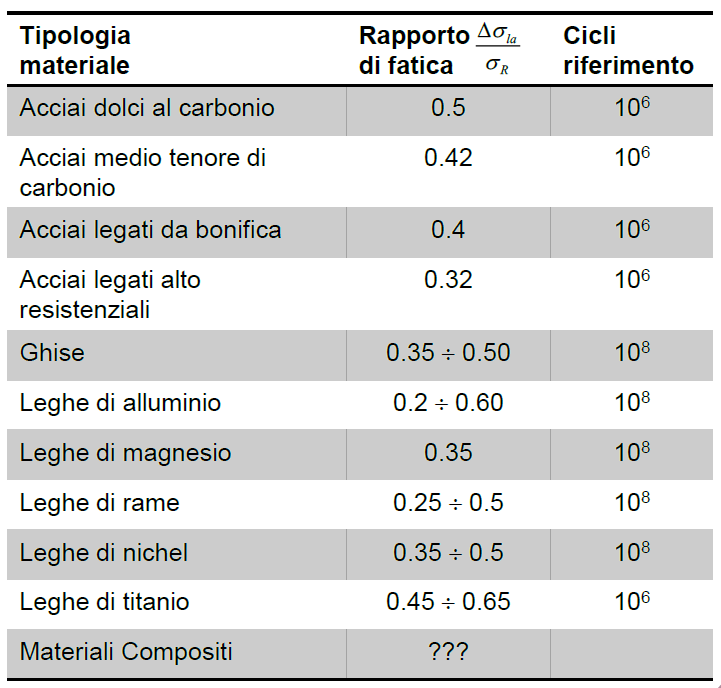
\includegraphics[width=0.3\linewidth]{fig/screenshot022}
			\label{fig:screenshot022}
		\end{figure}
		In questa figura le rette che si avvolgono senza strisciare sulla circonferenza sono $CT$ e $PB$, si nota subito infatti, che queste sono normali al profilo dell'evolvente e sono tangenti alla circonferenza fondamentale.
		
		\textbf{NB:} il punto di tangenza è sempre diverso lungo il profilo dell'evolvente,si muove mano a mano che ci si sposta lungo  il profilo.\newline  
		
		Da $A$ a $B$ l'inclinazione della normale all'evolvente rimane sempre la stessa che si individua nel punto C, centro di istantanea rotazione, ed è sempre l'angolo di pressione $\theta_0$ rispetto all'orizzontale.
		
		Tutti i punti sull'evolvente si possono tuttavia individuare attraverso l'angolo $\varphi$ formato dal segmento $PO$, distanza di un punto generico sull'evolvente dal centro della ruota ed il segmento $AO$, ed attraverso l'angolo $\theta$ (infelice scelta di nomi) tra il segmento $CO$ e $OT$, e poi tra il segmento $PO$ e $OB$, dove $OT=OB=\rho$ è il raggio della fondamentale; questo angolo varia mentre ci si sposta da $P$ ad $A$.
		
		In un sistema di riferimento cilindrico la posizione del generico punto $P$ diviene così nota attraverso due grandezze, l'anomalia $\varphi$ e la posizione radiale $\rho$.
	\end{adjustwidth}
	\subsection{Sviluppo dell'evolvente}
	\begin{adjustwidth}{2in}{}
		\textbf{Come si sviluppa un'evolvente per denti in successione?}
		\begin{figure}[H]
			\centering
			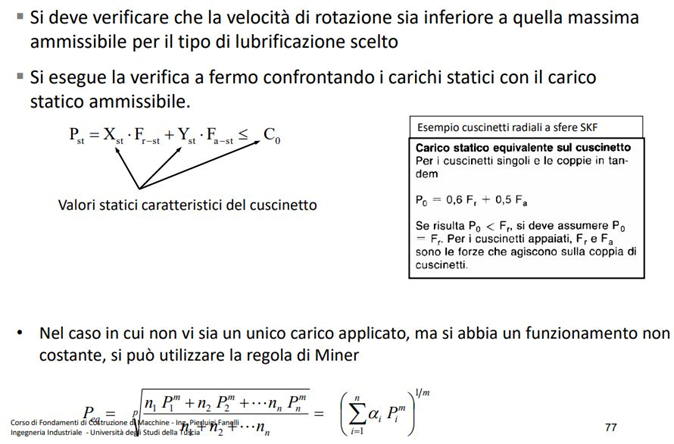
\includegraphics[width=0.5\linewidth]{fig/screenshot023}
			\label{fig:screenshot023}
		\end{figure}		
		La distanza che c'è tra due profili successivi è il passo trasversale, questo per definizione si misura come l'effettiva distanza tra due profili attivi secondo l'arco di circonferenza primitiva, tuttavia si può arrivare ad un'altra misura attraverso la definizione di evolvente, infatti questo profilo si ottiene inviluppando una retta su di una circonferenza fondamentale, in questo modo l'arco ottenuto una volta inviluppata la retta è proprio uguale a alla lunghezza della retta: questa distanza lineare è pari alla distanza ortogonale che c'è tra i profili, ed è uguale all'arco che andrebbe ad occupare quella retta.
		
		Per cui, proprio per proprietà dell'evolvente, la distanza ortogonale tra i due profili corrisponde al passo. 
		
		L'unica differenza consta nel fatto che il passo è misurato come arco di circonferenza primitiva, in questo modo però diviene misurabile come arco di circonferenza fondamentale (o di base), e quindi a parità di angolo la lunghezza dell'arco misurato sulla circonferenza fondamentale dell'evolvente sarà inferiore. 
		\begin{figure}[H]
			\centering
			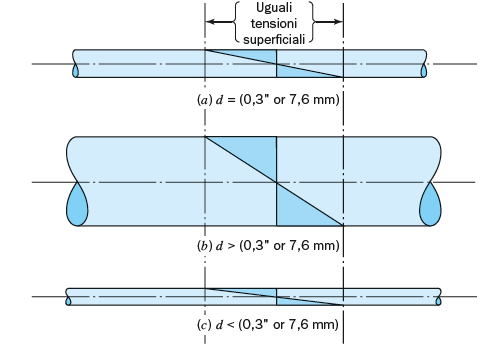
\includegraphics[width=0.3\linewidth]{fig/screenshot024}
			\label{fig:screenshot024}
		\end{figure}		
		Da quest'immagine si vede subito che il punto $P$ generico della evolvente (\textit{involute curve}) è dato dalla posizione $r$ e dall'angolo $\varphi$, quest'angolo è detto evolvente dell'anglo $\theta$  ed è una funzione matematica chiamata evolvente \[\varphi = \ev\theta\] (\textit{inv} in letteratura anglosassone).
\newpage		
		Ciò piega anche perché i profili siano coniugati: si vede infatti immediatamente, anche dalle figure precedenti, come i punti in contatto abbiano la normale in comune che punta sempre al centro di istantanea rotazione, invariate durante tutto l'ingranamento.
		
		Tale proprietà si conserva per qualsiasi ruota e per qualsiasi pignone.
		
		Infatti la costruzione dell'evolvente si ottiene in maniera del tutto indipendente su ruota e pignone - pur rispettando i paramenti geometrici - ed al montaggio garantisce che i profili siano sempre coniugati con un profilo che avrà un punto $P$ la cui normale è sempre tangente alla circonferenza fondamentale.
		
		Quando si vanno ad affiancare due ruote dal profilo ad evolvente queste avranno sempre profili coniugati.
\end{adjustwidth}
\subsubsection{Funzione evolvente}
\begin{adjustwidth}{2in}{}		
		\begin{figure}[H]
			\centering
			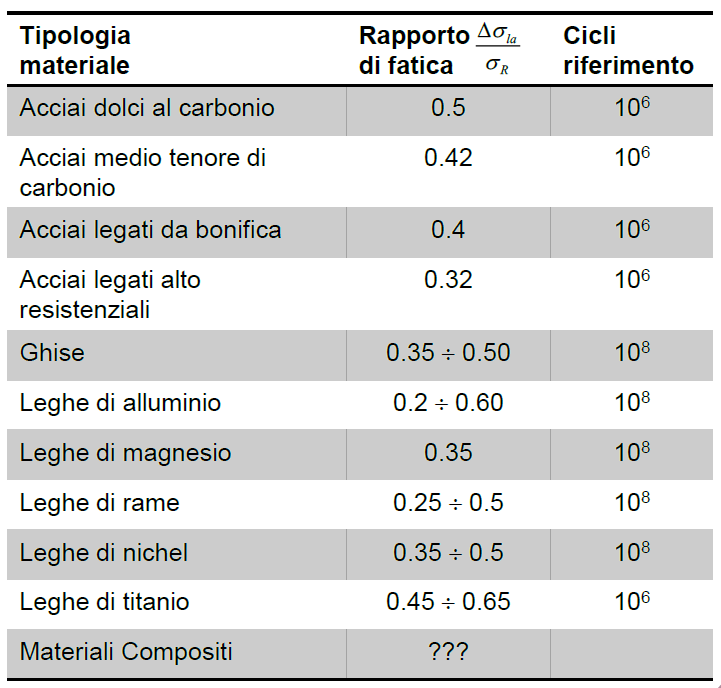
\includegraphics[width=0.5\linewidth]{fig/screenshot022}
			\label{fig:screenshot022_bis}
		\end{figure}
		L'anomalia $\varphi$, l'angolo che individua rispetto alla radice dell'evolvente $A$  la posizione angolare di $P$, sarà pari a
		\[\varphi = \hat{AOB}-\theta\]		
		Ci si pone come obiettivo l'identificazione di una funzione che prenda il posto di $\hat{AOB}$.\newline
		
		$B$ è il punto di tangenza alla circonferenza fondamentale della normale all'evolvente nel punto $P$.		
		Per definizione di evolvente la distanza $PB$ è assolutamente analoga all'arco $AB$ ciò significa che quel segmento, quando si avvolgerà senza strisciare sulla circonferenza fondamentale, porterà $P$ a coincidere con $A$
		\[PB=\overset{\frown}{AB}\]
		Per cui si può scrivere 
		\[\tan\theta = \dfrac{\sin\theta}{\cos\theta} \]
		Si ricordi a questo punto che l'angolo in B è retto, quindi per i triangoli rettangoli si può scrivere 
		\[\begin{dcases}
			PB = OP\sin\theta \Rightarrow \sin\theta = \dfrac{PB}{OP} \\
			OB = OP\cos\theta \Rightarrow \cos\theta = \dfrac{OB}{OP}
		\end{dcases}\]
		Per cui
		\[\tan\theta = \dfrac{PB}{OP}\dfrac{OP}{OB} = \dfrac{PB}{OB} \]
		$PB$ è noto mentre il tratto OB altro non è che il raggio della circonferenza di base della ruota $\rho$ 
		\[\tan\theta = \dfrac{PB}{OB}  = \dfrac{\overset{\frown}{AB}}{\rho}\]
		L'arco $\overset{\frown}{AB}$ è un arco che sottende un angolo $\hat{AOB}$ per cui la sua distanza lineare si può ottenere come 		
		\[\overset{\frown}{AB} = \rho\cdot\hat{AOB}\]
		Per cui
		\[\tan\theta = \dfrac{\rho\cdot\hat{AOB}}{\rho} = \hat{AOB}\]
		In questo modo si può così scrivere 
		\[\ev\theta=\varphi=\tan\theta-\theta\]
		E la posizione del punto P generico diviene così individuabile da 
		\[\varphi \qquad OP = \dfrac{\rho}{\cos\theta}\]
		\textbf{NB:} $\theta$ è una variabile angolare, non è l'angolo di pressione! \newline
		
		Quando sono in montaggio reciproco quell'angolo $\theta$ assume invece proprio il significato di angolo di pressione e allora i due profili ad evolvente qualunque sia l'interasse che assumono sono profili coniugati.
		
		Tuttavia cosa cambia al variare dell'interasse? Varia l'angolo di pressione e la circonferenza primitiva, mentre non varieranno né la circonferenza fondamentale né la forma del dente.
		
		Qual è la conseguenza della variazione dell'interasse? Variando l'angolo di pressione varieranno le forze scambiate tra i denti.
		
		Queste sono sempre orientate come la linea d'azione e hanno sempre due componenti: radiale e circonferenziale. Ai fini della trasmissione del moto la forza circonferenziale  - a meno di fluttuazioni di raggio di primitiva - rimane costante, mentre quella che varia è la componente radiale, infatti con un angolo di pressione maggiore si riscontra una maggiore componente radiale che sempre ai fini della trasmissione del moto è inutile, rappresenta soltanto un disturbo che sollecita maggiormente ed inutilmente albero e cuscinetti. 
		
		Spesso però l'interasse è un dato di progetto, ad esempio in un cambio di velocità lineare l'albero motore e l'albero condotto sono in una posizione relativa fissa qualunque sia la marcia che si sta innestando, significa che è su quei due assi che si devono realizzare gli ingranaggi delle marce, allora si dovrà giocare con le altre grandezze per ottenere un dimensionamento ottimale.
	\end{adjustwidth}
\newpage
\subsection{Raggio di curvatura - Teorema di Eulero-Savary}
	\begin{adjustwidth}{2in}{}
		\begin{figure}[H]
			\centering
			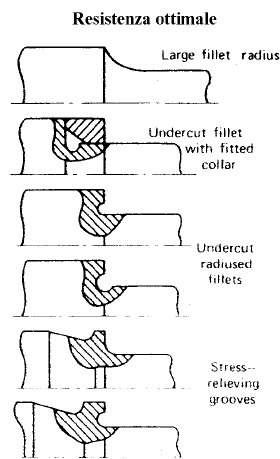
\includegraphics[width=0.5\linewidth]{fig/screenshot025}
			\label{fig:screenshot025}
		\end{figure}	
		La curvatura del profilo ad evolvente, ovvero la traiettoria che compie nel piano, è caratterizzata da un raggio di curvatura variabile: la curvatura in $A$ è diversa da quella in $C$ che è diversa da quella in $P$.
		
		Si vuole quantificare pertanto una funzione che quantifichi questo raggio di curvatura lungo l'evolvente. \newline
		
		\begin{thm}(Eulero-Savary)
		
			Dati due profili curvilinei, la differenza fra le curvature nel punto di contatto è data da
\begin{equation}\label{eq:el.sav}
				\dfrac{1}{R} - \dfrac{1}{R'} = \left(\dfrac{1}{C\Omega} - \dfrac{1}{CM}\right)\cos\beta
\end{equation}
			Dove
			\begin{itemize}
				\item \textbf{$R,R'$}: raggi di curvatura della polare fissa  \textbf{$p$}e della polare mobile \textbf{$p'$}, rispettivamente
				\item \textbf{$\Omega$}: centro di curvatura della rolletta descritta dal punto M solidale alla polare mobile
				\item \textbf{$\beta$}: angolo acuto formato dalla CM con la normale comune alle primitive in C.
			\end{itemize}
		\end{thm} 
		
		\textbf{Reminder}
		\begin{itemize}			
		\item La \textbf{polare fissa} è il luogo dei punti del piano solidale al riferimento fissato che nei successivi istanti diventano sede dei centri di istantanea rotazione del moto, cioè  sono quei punti in un piano fisso che sono destinati a diventare o sono stati centri di istantanea rotazione: per un cilindro che rotola senza strisciare sul piano la polare fissa è una linea sul piano.
		
		\item La \textbf{polare mobile} è simile alla polare fissa ma è pensata in un piano di riferimento mobile, è il luogo dei punti che durante il funzionamento diventeranno o sono stati centri di istantanea rotazione, cioè sono quei punti che durante il moto andranno a coincidere con i punti della polare fissa destinati ad essere centri di istantanea rotazione: sempre nel caso del cilindro che rotola sul piano, questi saranno i punti della circonferenza perché ciascuno di essi, in un certo istante del moto, diventerà centro di istantanea rotazione quando diventerà tangente. 
\newpage		
		\item $M$ è invece un punto descritto dalla \textbf{rulletta} della polare mobile. 
		
		Si immagini un cilindro rotolare su di un piano, si immagini di infilzarlo con uno spillo, la punta dello spillo percorre una certa traiettoria durante il rotolamento: la traccia del percorso di quella punta è la rulletta solidale alla polare mobile.
		
		In generale, per curve più complesse di quelle che possono essere rette o circonferenze, la traiettoria del punto M può essere più o meno complessa, per cui sovviene la necessità di definirne la curvatura.
		
		
		\item $M\Omega$ è il raggio di curvatura della rulletta descritta da $M$, per cui $\Omega$ è il centro di curvatura della rulletta passante per $M$, $O O'$ sono in centri di curvatura delle polari fisse e delle polari mobili nel punto di tangenza $C$ per sono allineati perché la normale ai profili dev'essere per definizione comune.
		
		\item $\beta$ è l'angolo che si instaura tra $CM$ e $CO$ o $CO'$.
	\end{itemize} 
	
		Le distanze sono prese tutte positive se ricadono dalla stessa parte della normale.
		\begin{figure}[H]
			\centering
			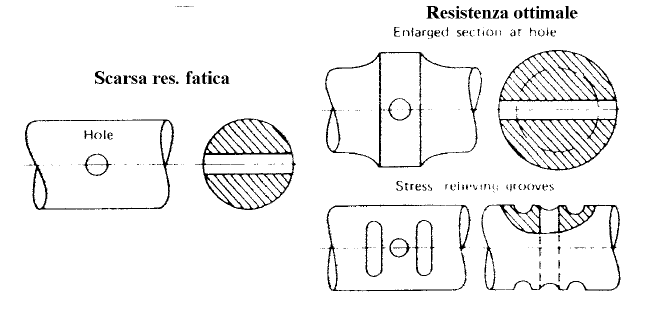
\includegraphics[width=0.5\linewidth]{fig/screenshot026}
			\label{fig:screenshot026}
		\end{figure}
	\end{adjustwidth}
	\subsubsection{Applicazione}
	\begin{adjustwidth}{2in}{}
		Si applichi questo teorema al profilo ad evolvente.
		
		Si vuole ricercare il centro di curvatura del punto $M$ quando questo è punto di contatto tra i profili $T$ e $T'$, questi, centri di curvatura del profilo nel punto $M$, con $T'$ centro coniugato.
		
		Per definizione di evolvente, questa altri non è che la rulletta di un punto della retta dei contatti che rotola senza strisciare sulla circonferenza fondamentale (il segmento dei contatti $TM$ che si avvolge sulla circonferenza fondamentale). 
		
		Per cui la polare mobile è la retta d'azione mentre la polare fissa è la circonferenza fondamentale rispettivamente centrata in $O$ e $'O$. \newline
		
		In $O$ l'angolo $\beta$ del teorema di Eulero-Savary è l'angolo tra $TM$ e la normale comune alle due polari in $T$ e quindi è un angolo tra la normale e la tangente: $\beta=90\degree$, in questo modo $\cos\beta=0$ tuttavia la differenza di curvatura non è nulla, per cui affinché la (\ref{eq:el.sav}) sia soddisfatta, occorre che il punto $T$ ($C$ nella notazione di (\ref{eq:el.sav})) di contatto fra le polari $\rho$ e $\rho'$ coincida con il centro di curvatura del profilo in $M$. 
\newpage		
		In questo modo $T$ rappresenta il centro di curvatura del profilo nel punto $M$ e $T'$ sarà parimenti il centro di curvatura del profilo coniugato sempre nel punto $M$, 
		
		Dalla figura, significa allora che $\Omega$ e $\Omega'$ sono i centri di curvatura del profilo durante tutto l'ingranamento e quindi per proprietà dell'evolvente i punti di contatto tra un dente e l'altro, punti che cambiano istante per istante lungo il profilo, sono tutti caratterizzati dallo stesso centro di curvatura durante tutto l'ingranamento.\newline 
		
		Il generico punto di contatto dista dal centro di istantanea rotazione $C$, una quantità $\delta$ variabile durante l'ingranamento, per cui i raggi di curvatura dei profili $\Omega M$ ed $M\Omega'$ si possono scrivere come 
		\[\Omega M = \Omega C +CM = \rho\cdot\tan\theta + \delta = R\cos\theta\cdot\dfrac{\sin\theta}{\cos\theta} + \delta = R\sin\theta +\delta\]
		Analogamente 
		\[M\Omega' = R'\sin\theta-\delta\]		
		Queste due quantità sommate tra loro rappresentano la distanza dei centri di curvatura 
		\[\Omega\Omega' = \sin\theta(R+R')\] 				
		Tale grandezza è costante ed indipendente dal punto di ingranamento: d'altro canto è la distanza tra i punti di tangenza della retta d'azione e rappresenta anche ciò che all'inizio si è definito come segmento teorico massimo dei contatti, è la distanza che si misura tra il punto del profilo ad evolvente massimo realizzabile - quello sulla circonferenza fondamentale della ruota - e quello sulla circonferenza fondamentale del pignone, quando questi assumono una posizione di possibile contatto. 
\end{adjustwidth}

\section{Proporzionamento modulare}		
\begin{adjustwidth}{2in}{}			
		Il numero di denti e la dimensione del dente in una ruota dentata è sempre proporzionale ad un numero, si parla infatti di ruote dentate a proporzionamento modulare ovvero sia l'addendum e il dedendum cosi come il diametro della ruota, il passo e tutte le grandezze geometriche d'interesse dipendono da un numero $m = [\si{\milli\meter}]$. \newline 
		
		Si era definito il modulo come il rapporto tra il valore del diametro della circonferenza primitiva ed il numero di denti
		\[m = \dfrac{2R}{z}\]		
		In funzione del modulo così individuato si andrà a proporzionare l'altezza del dente, infatti per il pignone l'addendum sarà pari a 
		\[a = k \cdot m\] 
		Ed il dedendum a
		\[u = k^* \cdot m\]
		Con $k$ e $k^*$  scalari dipendenti dal tipo di proporzionamento adottato. \newline 
		
		Per motivi legati all’interferenza nell’ingranamento, diverrà necessario considerare l’effetto che ha l’addendum della ruota coniugata con la ruota che si sta considerando, pertanto il parametro fondamentale di
		proporzionamento a cui spesso ci si riferirà sarà $k’$ essendo per la ruota
		\[a' = k' \cdot m\]
\newpage				
		Due ruote coniugate affinché sia valido l'accoppiamento devono avere lo stesso modulo e ciò mette a riparo da numerosi problemi. 
		
		La realizzazione delle ruote dentate infatti è standardizzata in funzione del modulo, così come le dimensioni del dente e della ruota: una ruota dentata si sostituisce solo con una ruota dentata dello stesso modulo. \newline
				
		$k, k'$ e $k^*$ sono coefficienti anch'essi normalizzati e standardizzati e forniscono l'aspetto finale della dentatura, dicono infatti quanto il dente deve sporgere (addendum) e quanto deve rientrare (dedendum), la somma di addendum e dedendum darà l'altezza del dente e quindi in funzione di quanto varranno questi coefficiente si avranno dentature magari più allungate, con maggior fattore di ricoprimento e con dente più sottile, tuttavia c'è da notare che un dente di una ruota dentata è perfettamente schematizzabile come una trave a mensola incastrata che subisce un carico ortogonale e di compressione, per cui va da se che ad una base più sottile si associa una resistenza minore e viceversa.
		
		Inoltre il proporzionamento dev'essere tale che l'addendum di una ruota sia sempre inferiore al dedendum dell'altra: c'è sempre del \textbf{gioco radiale} fra la testa di un dente e il piede del dente della ruota coniugata.\newline 
		
		
		\textbf{Si può misurare la circonferenza primitiva di una ruota?} 
		
		Sul piano frontale si possono individuare il raggio di testa (distanza radiale dal centro alla testa del dente) ed il raggio di piede, se sono sufficientemente grandi si possono anche osservare i raggi di curvatura e quindi le troncature esterne ed interne, ma la primitiva è una grandezza cinematica di funzionamento e di montaggio e non può mai essere misurata fisicamente. 
		
		Si può misurare anche l'altezza del dente, questa somma di addendum e dedendum, ma non i singoli addendum e dedendum ricavabili solo matematicamente. 
		
		In ogni caso, in questa fase, l'importante è che il dendendum sia maggiore dell'addendum in modo da garantire un gioco radiale tra la testa del dente ed il piede di quello coniugato, perché se cosi non fosse, durante l'ingranamento la testa del pignone "entrerebbe" dentro la ruota coniugata, con interferenza e bloccaggio istantaneo dell'ingranamento. 
		
		Per evitare ciò, il $k^*$ del pignone dev'essere maggiore del $k'$  della ruota e viceversa: il dente deve sporgere meno di quanto rientra quello coniugato.
\end{adjustwidth}
\subsection{Realizzazione}
\begin{adjustwidth}{2in}{}		
		Gli aspetti tecnologici saranno dettagliatamente vagliati in futuro, per ora interessa sapere che esistono principalmente due metodi di realizzazione delle ruote dentate
		\begin{itemize}
			\item Per fresatura: si fresa il vano tra due denti con una fresa a disco o a bottone. 
			
			Laborioso e costoso, è necessaria una fresa per ogni tipologia di ruota.
			
			\item Dentiera, Creatore, Ruota Fellows: sfruttano l'accoppiamento cinematico per realizzare la ruota dentata.
		\end{itemize} 
		Per ruote dentate standard normalmente si utilizza la dentiera, infatti l'obiettivo della realizzazione è l'ottenimento di una dentatura ad evolvente, questa si ricava tramite l'accoppiamento cinematico di una polare mobile (una retta), che si avvolge su una polare fissa (una circonferenza). \newline 
		
		Il moto delle polari tuttavia non dev'essere per forza assoluto, può essere anche relativo, infatti una retta che si avvolge su una circonferenza, che questa ruoti o meno, porta sempre alla generazione di un evolvente: è esattamente questo il modo con cui si sviluppano le ruote dentate, la primitiva del rocchetto rotola senza strisciare su una retta individuata dalla dentiera, se su questa si pongono una serie di punti fisici che altro non sono che i denti taglienti della dentiera, ciascuno di questi punti nel moto di accoppiamento con la circonferenza primitiva del rocchetto descrive un evolvente.
\newpage
		\begin{figure}[H]
			\centering
			\includegraphics[width=0.5\linewidth]{fig/creatrice}
			\label{fig:creatrice}
		\end{figure}
		In questo modo la superficie che si ottiene per sottrazione successiva di materiale da parte dei denti della dentiera è nient'altro che i denti della ruota dentata realizzata, vuol dire che la forma finale dell'evolvente è dettata dalla forma dei denti della dentiera. \newline
		
		L'altezza finale del dente è uguale all'altezza del dente della dentiera senza però considerare il gioco radiale.
		
		In un proporzionamento modulare se $(k+k^*)m$ è la somma di addendum e dedendum, questa sarà per forza anche l'altezza del dente della dentiera. 
		
		In più proprio per proprietà dell'evolvente, la dentiera avrà un profilo perfettamente rettilineo perché in ogni caso l'accoppiamento darà sempre luogo ad una dentatura ad evolvente. \newline
		
		Il grande vantaggio nel realizzare per inviluppo una ruota dentata è che in questo modo è necessario conoscere solamente il valore del modulo: la stessa dentiera con $m=\SI{2}{\milli\meter}$ si può utilizzare per realizzare una ruota dal diametro di \SI{30}{\milli\meter} con 15 denti, o una dal diametro di \SI{60}{\milli\meter} con 30 denti. 
		
		La forma del dente di quella da \SI{60}{\milli\meter} sarà chiaramente diversa da quella della ruota da \SI{30}{\milli\meter}, ma per fresatura avrei avuto bisogno di due diversi utensili per realizzarle.\newline
		
		L'angolo di pressione si ritrova come l'inclinazione fra la normale al profilo della dentiera e l'orizzontale sulla primitiva di riferimento della dentiera. 
		
		Se la dentiera è fatta come in figura sotto, sulla ruota realizzata l'angolo di pressione sarà sempre pari a 20\degree. 
		\begin{figure}[H]
			\centering
			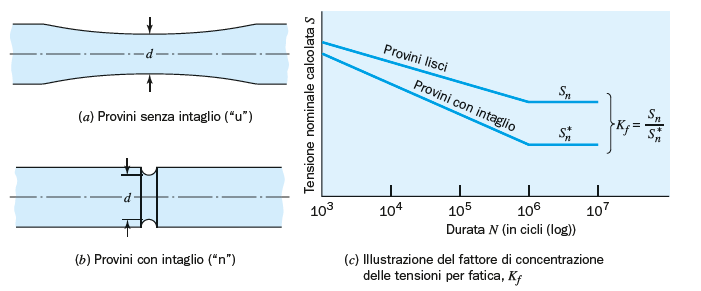
\includegraphics[width=0.9\linewidth]{fig/screenshot027}
			\label{fig:screenshot027}
		\end{figure}		
		\textbf{Come sono fatti i raccordi e la testa del dente?} 
		
		Il profilo effettivo di contatto ad evolvente è compreso tra il raggio di piede, di solido mai superiore a $0.4m$, e la spoglia di testa, questa solitamente molto piccola, serve infatti esclusivamente a ridurre i problemi di impuntamento e di intaglio e non si superano mai valori come lo $0.02m$ in direzione circonferenziale e lo $0.06m$ in direzione radiale.
\end{adjustwidth}
\newpage
\subsection{Proporzionamento Normale Unificato}
\begin{adjustwidth}{2in}{}					
		Il proporzionamento utilizzato più frequentemente ad oggi è quello normale unificato e prevede \[k=1\] Per cui l'addendum è pari al modulo \[a=m\] Una ruota di modulo 2 vuol dire che ha un dente che sporge di \SI{2}{\milli\meter} rispetto alla primitiva. \newline 
		
		Il dedendum invece è pari a \[u = 1.25m\] Ed è uguale per ruota e pignone: d'altronde tale distinzione è il progettista a darla, la proprietà dell'evolvente permette in ogni caso di montarle come si vuole, purché abbiano lo stesso modulo. \newline 
		
		La dentiera di riferimento in base alla quale è compiuto questo proporzionamento è caratteristica di un angolo
		di pressione pari a 20\degree. \newline
		
		Il gioco radiale, lo spazio tra la testa del dente del pignone e il piede del dente della ruota, è pari a \[g = u-a = 0.25m\] Il gioco radiale è importante per
		\begin{itemize}
			\item Garantire un ottimale passaggio di lubrificante;
			\item Evitare l'interferenza di evolvente e di piede
			\begin{itemize}
				\item Interferenza di evolvente: il dente viene spinto così radialmente in avanti che tocca contemporaneamente il profilo utile e quello ozioso della ruota coniugata;
				\item Interferenza di piede: la testa di una ruota tocca il piede dell'altra
			\end{itemize}
			
		\end{itemize} 
\end{adjustwidth}
\subsection{Proporzionamento Tradizionale}
\begin{adjustwidth}{2in}{}			
		Un altro tipo di proporzionamento viene comunemente chiamato tradizionale e prevede un addendum sempre pari al modulo \[a=m\]  Ma un dedendum pari a \[u = \dfrac{7}{6}m\] Il risultato è che l'altezza del dente diviene pari a \[h = \dfrac{13}{6}\] Ed è minore dell'altezza ottenuta col metodo normale. \newline
		
		\textbf{Perché dovrebbe essere preferita un altezza del dente minore?} 
		
		Meno ingombro, una trasmissione più compatta, di contro si avrà una riduzione del fattore di ricoprimento e del gioco radiale
		\[g = u-a = 0.167m\]		
		Esistono poi altri proporzionamenti, come quello tedesco che prevede un dente molto ribassato e robusto, con un ingombro ridotto ma con un fattore di ricoprimento, e quindi un'efficienza, minori. \newline
		 
\begin{center}
	\textbf{Qualora non specificato, si parlerà sempre di proporzionamento normale unificato.} \newline
\end{center}
\end{adjustwidth}
\subsection{Spessore del dente I}
\begin{adjustwidth}{2in}{}		
		Per risolvere il problema di \textbf{interferenza di evolvente} si deve porre particolare attenzione al fatto che la condizione di ingranamento prevede al massimo che la somma dei due \textbf{spessori} del dente su pignone e ruota sia uguale al passo.
		
		Cioè lungo la circonferenza primitiva se si misura lo spessore del dente della ruota e lo spessore del dente del pignone, sommati devono restituire il passo, altrimenti ci si troverà in condizione di interferenza: o non entra il dente dentro il vano, o il moto è discontinuo.
		\[s'+s = p\]		
		Nei proporzionamenti visti fin'ora lo spessore del dente di ruota e di pignone sono identici
		\[s'= s\] 
		Per cui si ottiene una relazione che lega lo spessore del dente al \textbf{semipasso} ovvero allo spessore nominale del dente misurato sulla primitiva
		\[2s = p \Rightarrow \dfrac{p}{2}-s=0\]
		Tale differenza non si pone mai esattamente pari a zero perché in questo modo il dente toccherebbe contemporaneamente sia il profilo ozioso che il profilo attivo della ruota coniugata, quindi nella pratica costruttiva lo spessore del dente sarà sempre leggermente più piccolo del vano in modo che durante l'ingranamento si tocchi solamente il profilo attivo, in questo modo la relazione della somma degli spessori diviene
		\[\dfrac{p}{2}-s>0\]
		Inoltre sarà necessario tenere conto sia della lubrificazione - avere uno spazio in direzione circonferenziale permette di far fluire lubrificante - sia della generazione di calore per attrito che tende a dilatare il dente nelle due direzioni principali, nonché di eventuali imprecisioni di montaggio e deflessioni degli alberi.\newline 
		
		Nel proporzionamento cinematico e tale differenza si prenderà pari a zero come sola condizione di ingranamento
		\[{p\over2}-s=0\] A posteriori si andrà a correggere per garantire la lubrificazione e la risoluzione dei problemi citati. 
\end{adjustwidth}
\subsection{Profili}
\begin{adjustwidth}{2in}{}			
		La parte di profilo che interessa per definire l'ingranamento è quella compresa tra la troncatura esterna e la troncatura interna, individuate dalle rispettive circonferenze al netto del raggio di curvatura di piede e dell'angolo di spoglia in testa. \newline 
		
		\textbf{Perché è necessario definire queste grandezze?} Perché al di spora della troncatura esterna l'angolo di spoglia non segue l'evolvente e quindi non può essere profilo di contatto, mentre al di sotto della troncatura interna il raggio di piede non è un profilo ad evolvente e quindi neanche questo può prendere parte al contatto.
		\begin{figure}[H]
			\centering
			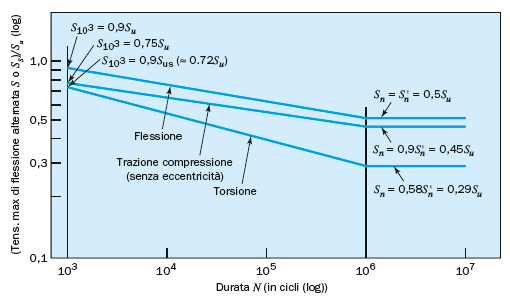
\includegraphics[width=0.7\linewidth]{fig/screenshot028}
			\label{fig:screenshot028}
		\end{figure}		
		Se tra troncatura esterna e troncatura interna il profilo è ad evolvente si ha la certezza che la circonferenza di base è minore della troncatura interna. Se così non fosse e la circonferenza di base (circonferenza da cui viene generata l'evolvente, fondamentale) fosse più alta cadendo all'infuori del cerchio di piede, ovvero tra le due troncature, il profilo di evolvente, quello efficace al contatto, sarebbe molto minore e si arriverebbe prima alla troncatura esterna mentre la troncatura interna non è più dettata dal raggio di raccordo bensì dalla circonferenza di base conducendo a chiari fenomeni di interferenza.
		
		I raccordi di testa e di piede, nel caso di realizzazione per fresatura, devono essere realizzati sagomando opportunamente l'utensile, questo infatti è sempre il negativo del dente, la forma del vano finale. Quando invece si realizza per inviluppo, la dentiera utensile non ha la stessa forma della ruota dentata finale e allora per ottenere i raggi di raccordo basterà darle una particolare forma, se infatti questa si scosta dal tratto rettilineo durante il cinematismo di taglio, genererà delle curve che sono rullette diverse dall'evolvente ottenendo in questo modo i raggi di raccordo desiderati.	
\end{adjustwidth}
\subsubsection{Osservazione}
\begin{adjustwidth}{2in}{}		
		Se si immagina una condizione di ingranamento con un profilo completamente ad evolvente e la circonferenza di base coincidente con quella di piede, tutto il profilo è ad evolvente.
		
		La parte di evolvente subito sopra al raggio di raccordo del piede è una parte di evolvente utile al contatto, tuttavia spingersi vicino alla circonferenza di base non è per nulla auspicabile perché il contatto in quella zona, molto lontana dalla circonferenza primitiva, porta a maggiori strisciamenti dovuti al semplice fatto che le velocità periferiche sono diverse.
		
		Tant'è che spesso si preferisce evitare del tutto il contatto in quella zona raccordando internamente il dente o asportandone una parte, in questo modo quando arriva la ruota coniugata che vorrebbe dar luogo al contatto, non trova nulla.
		
		Si perde parte del segmento dei contatti e si riduce il fattore di ricoprimento, ma si evita il contatto in un punto estremamente pericoloso. Questa è una scelta che deve essere giustamente ponderata perché perdendo fattore di ricoprimento si rischia di andare in condizioni di non continuità del moto, in più, si è ridotta anche la sezione resistente del dente. \newline
		
		(Qual è il giusto raggio di raccordo se si realizza la ruota dentata per fresatura? La geometria che deve essere realizzata può essere data dal raccordo di Schiebel EXTRA sul \textit{Giovannozzi}. 
		
		NUOVO FILE PER Schiebel Parte 16)
\newpage
		
		Il profilo che si ottiene per inviluppo è l'inviluppo delle posizione della dentiera istante per instante durante l'inviluppo.
		\begin{figure}[H]
			\centering
			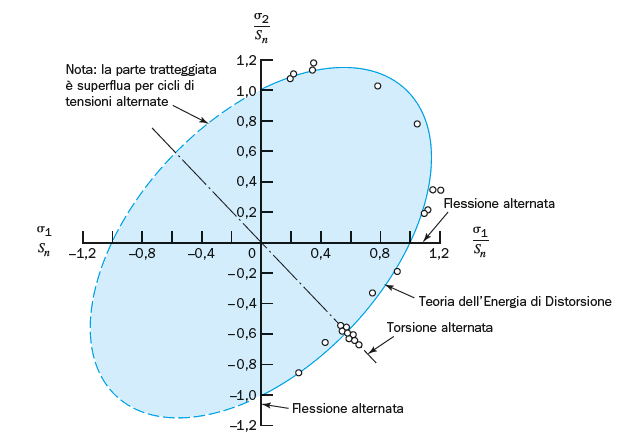
\includegraphics[width=0.7\linewidth]{fig/screenshot029}
			\label{fig:screenshot029}
		\end{figure}		
		La forma del dente della dentiera si intravede nei tracciati, e rotolando senza strisciare su una circonferenza di base che ruota, genera ad ogni passata questo profilo. 
		 
		La dentiera contiene in sè informazioni sul modulo sull'angolo di pressione, quest'ultimo in un proporzionamento normale è solitamente pari a 20\degree e raramente esistono casi in cui si utilizzano angolo di pressione di 22\degree 25\degree 30\degree: se cambia l'angolo di pressione infatti cambia l'aspetto del dente; in figura si vede il dente a punta, come se fosse una picca, se si va ad aumentare l'angolo di pressione il dente diventa molto più largo alla base - e quindi più robusto - ma la dimensione circonferenziale però non varia la ruota ha quella circonferenza e quindi diminuisce giocoforza il numero di denti che si possono realizzare. 
		 
		Un altro problema relativo all'aumento dell'angolo di pressione è la diminuzione dello spessore in testa, questo fatto porta a maggiori probabilità che deformazioni, cattivi montaggi o vibrazioni portino ad impuntamenti della testa durante l'ingranamento con rischio di deformazioni dell'albero. 
\end{adjustwidth}		 
		\begin{figure}[H]
			\centering
			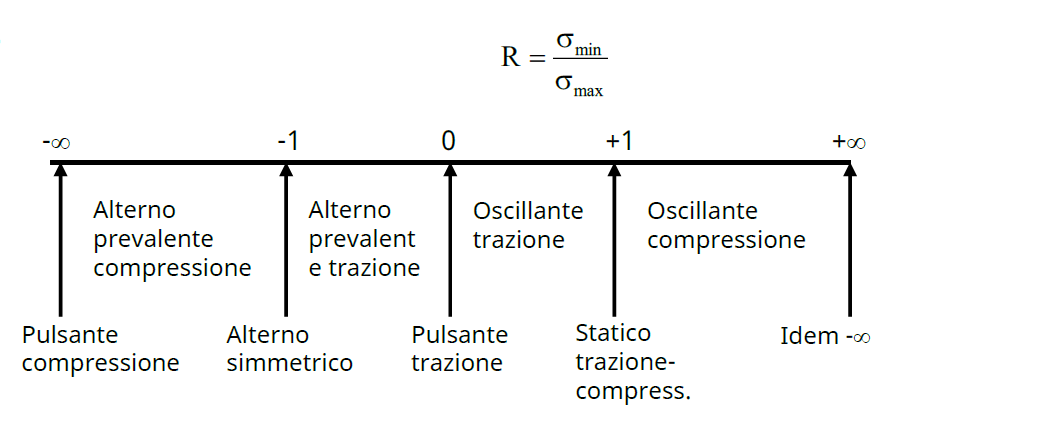
\includegraphics[width=0.5\linewidth]{fig/screenshot030}
			\caption{Inviluppo di una ruota dentata completa}
			\label{fig:screenshot030}
		\end{figure}
\newpage
\subsection{Spessore del dente II}
\begin{adjustwidth}{2in}{}			
		Lo spessore del dente serve ad individuare la condizione di ingranamento, diviene così necessario identificare una relazione matematica che fornisca l'esatto spessore del dente ad evolvente, anche alla luce del fatto che in testa deve essere sufficientemente grande ed in funziona di quanto vale alla base fornisce un valore resistenziale.
		\begin{figure}[H]
			\centering
			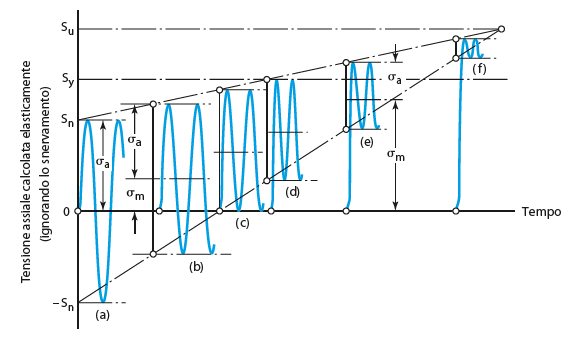
\includegraphics[width=0.7\linewidth]{fig/screenshot031}
			\label{fig:screenshot031}
		\end{figure}		
		Si immagini un dente cosi rappresentato, che si estende ad $A$ ad $A'$.
		
		Sia un punto $P$ sull'evolvente rispetto al quale si misura lo spessore $s$ e un punto $P^*$ in cui si misura lo spessore $s^*$. 
		
		Lo spessore si misura sempre in archi di circonferenza per cui ad $s^*$ si associa l'arco di raggio $OP^*$ e ad $s$ si associa l'arco di raggio $OP$.
		
		Si vuole conoscere $s^*$ a partire dal valore di $s$. \newline 
		
		Si individua l'angolo $\hat{POP^*}$ come l'angolo ottenuto sull'evolvente in diversi punti successivi, infatti osservando la figura si ottiene 
		\[\varphi = \hat{AOP} \qquad \varphi^* = \hat{AOP^*}\] 
		Ricordando il rapporto tra l'anomalia e la funzione evolvente si ha
		\[\hat{POP^*} = \varphi^*-\varphi = \ev\theta^*-\ev\theta\] 
		
		$OP^*$ è la posizione radiale del punto rispetto al quale si vuole calcolare lo spessore, questa quantità altro non è che, in funzione del raggio di fondamentale $\rho$
		\[OP^* = r^* = \dfrac{\rho}{\cos\theta^*}\] 
		Similmente $OP$ è la posizione radiale del punto rispetto al quale si conosce lo spessore
		\[OP = r = \dfrac{\rho}{\cos\theta}\] 		
		Lo spessore $s^*$ è un arco che sottende un angolo $\hat{P^*OQ^*}$, se questo viene moltiplicato per il raggio $OP^*$, si ottiene l'esatto valore dello spessore $s^*$
		\[s^* = \hat{P^*OQ^*}\cdot r^*\] 
		Dalla figura si evince che 
		\[\hat{P^*OQ^*} = POQ - 2POP^*\] 
		Si può sempre mettere in relazione l'arco con il raggio e il suo angolo sotteso, per cui
		\[\hat{P^*OQ^*} = \dfrac{s^*}{r^*}\qquad\hat{POQ} = \dfrac{s}{r}\]
		E quindi
		\[\hat{P^*OQ^*} = POQ - 2POP^*\]
		\[\dfrac{s^*}{r^*} = \dfrac{s}{r} - 2POP^*\]
		\[s^* = r^*\left[\dfrac{s}{r} - 2(\ev\theta^*-\ev\theta)\right]\]
		Equivalentemente, cambiando di segno
		\begin{equation}\label{eq:1}
			s^* = r^*\left[\dfrac{s}{r} + 2(\ev\theta-\ev\theta^*)\right]
		\end{equation}
		Questa è la relazione che fornisce un valore di spessore ad una certa quota radiale rispetto allo spessore ad un'altra quota radiale noto.\newline 
		
		Se si vuole trovare lo spessore in termini assoluti, allora si deve fissare un $s$ noto valutandolo in un punto particolare: la punta
		\[s(V) = 0\] 
		In questo modo la relazione (\ref{eq:1}) diviene
		\[s^* = 2r^*(\ev\theta-\ev\theta^*)\] 
		Ma $\ev\theta$ cos'è? Prima era l'anomalia $\varphi$ del punto $P$, ora che si è un $V$, sarà l'anomalia del punto $V$ che, dall'immagine, viene identificata dall'angolo $\gamma$ ovvero $\ev\gamma$, semiampiezza del dente. \newline  
		
		Allora lo spessore del dente in un qualunque punto $P^*$ è pari a 
		\[s^* = 2r^*(\ev\gamma-\ev\theta^*)\]  
		Con $r^*$ posizione radiale che si sta ricercando. 
		
		
		\textbf{!ATTENZIONE!}: Questo $\theta^*$ non è l'angolo di pressione, ma è la variabile dell'evolvente! \newline
		
		Come si ricava  l'evolvente di $\gamma$? Particolarizzando la relazione in un punto che magari già si conosce.
		
		Ad esempio spesso si conosce lo spessore alla base e quindi da tale formula si può estrapolare l'evolvente di gamma
		\[s_b = 2\rho\cdot\ev\gamma = 2R\cos\theta_0\cdot\ev\gamma\] 
		Oppure lo si conosce dalla primitiva, e quindi si particolarizza tale equazione sulla primitiva: in ogni caso $\ev\gamma$ si ricava sempre da uno spessore noto ad una determinata quota.
		    
	     
	     
		
		
	    
 
	    
	    
	    
	    
	    
	   
	     
	     
	     
	     
	
	
	
	
	
	
	
	
	
	
	
	
	
	
	
	
	\newpage
	\textbf{{\LARGE NOTE}}
%	\vfill
%	\begin{tcolorbox}[height=4.5cm]
%		This box has a height of 4.5cm.
%	\end{tcolorbox}
	
	%DA DECOMMENTARE PER AVERE LA VERSIONE STAMPABILE A DUE PAGINE 	
	%	\newpage
	%		\null
	%		\vfill
	%\begin{tcolorbox}[height=4.5cm]
	%	This box has a height of 4.5cm.
	%\end{tcolorbox}
	%		
\end{adjustwidth}
\end{document}